\documentclass[letterpaper,USenglish,cleveref, autoref, thm-restate]{lipics-v2021}
%This is a template for producing LIPIcs articles.
%See lipics-v2021-authors-guidelines.pdf for further information.
%for A4 paper format use option "a4paper", for US-letter use option "letterpaper"
%for british hyphenation rules use option "UKenglish", for american hyphenation rules use option "USenglish"
%for section-numbered lemmas etc., use "numberwithinsect"
%for enabling cleveref support, use "cleveref"
%for enabling autoref support, use "autoref"
%for anonymousing the authors (e.g. for double-blind review), add "anonymous"
%for enabling thm-restate support, use "thm-restate"
%for enabling a two-column layout for the author/affilation part (only applicable for > 6 authors), use "authorcolumns"
%for producing a PDF according the PDF/A standard, add "pdfa"

%\pdfoutput=1 %uncomment to ensure pdflatex processing (mandatatory e.g. to submit to arXiv)
%\hideLIPIcs  %uncomment to remove references to LIPIcs series (logo, DOI, ...), e.g. when preparing a pre-final version to be uploaded to arXiv or another public repository

%\graphicspath{{./graphics/}}%helpful if your graphic files are in another directory

\usepackage{amsmath}
\usepackage{tikz}
\usepackage{pgfplots}
\usepackage{booktabs}
\usepackage{hyperref}

\newcommand{\pand}{\mathbin{\land^{\sf p}}}
\newcommand{\por}{\mathbin{\lor^{\sf p}}}
\DeclareMathOperator*{\Pand}{\bigwedge^{\sf p}}
\DeclareMathOperator*{\Por}{\bigvee^{\sf p}}
\newcommand{\boolnot}{\neg}
\newcommand{\tautology}{\top}
\newcommand{\nil}{\bot}
\newcommand{\obar}[1]{\overline{#1}}
\newcommand{\oneminus}{{\sim}}
\newcommand{\lit}{\ell}

\newcommand{\varset}{X}
\newcommand{\exvarset}{Z}
\newcommand{\dependencyset}{{\cal D}}
\newcommand{\litset}{{\cal L}}
\newcommand{\ring}{{\cal R}}
\newcommand{\dset}{{\cal A}}
\newcommand{\rep}{\textbf{R}}
\newcommand{\radd}{+}
\newcommand{\rmul}{\times}
\newcommand{\addident}{\textbf{0}}
\newcommand{\mulident}{\textbf{1}}
\newcommand{\imply}{\Rightarrow}
\newcommand{\ifandonlyif}{\Leftrightarrow}
%\newcommand{\drational}{\mathbb{Q}_{2,5}}
\newcommand{\drational}{\textbf{Q}_{2,5}}

\newcommand{\assign}{\alpha}
\newcommand{\passign}{\rho}
\newcommand{\lassign}{\beta}
\newcommand{\uassign}{{\cal U}}
\newcommand{\modelset}{{\cal M}}

\newcommand{\indegree}{\textrm{indegree}}
\newcommand{\outdegree}{\textrm{outdegree}}
\newcommand{\validate}{\textsf{validate}}
\newcommand{\prov}{\textrm{Prov}}
\newcommand{\inputformula}{\phi_I}
\newcommand{\pogformula}{\theta_P}

\newcommand{\makenode}[1]{\mathbf{#1}}
\newcommand{\nodeu}{\makenode{u}}
\newcommand{\nodev}{\makenode{v}}
\newcommand{\nodes}{\makenode{s}}
\newcommand{\nodep}{\makenode{p}}
\newcommand{\noder}{\makenode{r}}

\newcommand{\simplify}[2]{#1|_{#2}}

\newcommand{\progname}[1]{\textsc{#1}}
\newcommand{\dfour}{\progname{D4}}
\newcommand{\Dfour}{\progname{D4}}
\newcommand{\cadical}{\progname{CaDiCal}}
\newcommand{\dtrim}{\progname{drat-trim}}

\definecolor{redorange}{rgb}{0.878431, 0.235294, 0.192157}
\definecolor{lightblue}{rgb}{0.552941, 0.72549, 0.792157}
\definecolor{clearyellow}{rgb}{0.964706, 0.745098, 0}
\definecolor{clearorange}{rgb}{0.917647, 0.462745, 0}
\definecolor{mildgray}{rgb}{0.54902, 0.509804, 0.47451}
\definecolor{softblue}{rgb}{0.643137, 0.858824, 0.909804}
\definecolor{bluegray}{rgb}{0.141176, 0.313725, 0.603922}
\definecolor{lightgreen}{rgb}{0.709804, 0.741176, 0}
\definecolor{darkgreen}{rgb}{0.152941, 0.576471, 0.172549}
\definecolor{redpurple}{rgb}{0.835294, 0, 0.196078}
\definecolor{midblue}{rgb}{0, 0.592157, 0.662745}
\definecolor{clearpurple}{rgb}{0.67451, 0.0784314, 0.352941}
\definecolor{browngreen}{rgb}{0.333333, 0.313725, 0.145098}
\definecolor{darkestpurple}{rgb}{0.396078, 0.113725, 0.196078}
\definecolor{greypurple}{rgb}{0.294118, 0.219608, 0.298039}
\definecolor{darkturquoise}{rgb}{0, 0.239216, 0.298039}
\definecolor{darkbrown}{rgb}{0.305882, 0.211765, 0.160784}
\definecolor{midgreen}{rgb}{0.560784, 0.6, 0.243137}
\definecolor{darkred}{rgb}{0.576471, 0.152941, 0.172549}
\definecolor{darkpurple}{rgb}{0.313725, 0.027451, 0.470588}
\definecolor{darkestblue}{rgb}{0, 0.156863, 0.333333}
\definecolor{lightpurple}{rgb}{0.776471, 0.690196, 0.737255}
\definecolor{softgreen}{rgb}{0.733333, 0.772549, 0.572549}
\definecolor{offwhite}{rgb}{0.839216, 0.823529, 0.768627}
\definecolor{medgreen}{rgb}{0.15, 0.6, 0.15}

% Lean code:
\usepackage{listings}
%\definecolor{keywordcolor}{rgb}{0.7, 0.1, 0.1}   % red
\definecolor{keywordcolor}{rgb}{0.0, 0.1, 0.6}   % blue
\definecolor{tacticcolor}{rgb}{0.0, 0.1, 0.6}    % blue
\definecolor{commentcolor}{rgb}{0.4, 0.4, 0.4}   % grey
\definecolor{symbolcolor}{rgb}{0.0, 0.1, 0.6}    % blue
\definecolor{sortcolor}{rgb}{0.1, 0.5, 0.1}      % green
\definecolor{attributecolor}{rgb}{0.7, 0.1, 0.1} % red
\def\lstlanguagefiles{lstlean.tex}
% set default language
\lstset{language=lean, xleftmargin=1em}
\lstset{backgroundcolor=\color{white}}

\bibliographystyle{plainurl}% the mandatory bibstyle

\title{Certified Knowledge Compilation \\ with Application to Verified Model Counting}

\titlerunning{Certified Knowledge Compilation}

\author{Randal E. Bryant}{Computer Science Department, Carnegie Mellon University, Pittsburgh, PA 15213 USA}{rebryant@cmu.edu}{https://orcid.org/0000-0001-5024-6613}{Supported by NSF grant CCF-2108521}
\author{Wojciech Nawrocki}{Department of Philosophy, Carnegie Mellon University}{wjnawrock@cmu.edu}{https://orcid.org/0000-0002-8839-0618}{}
\author{Jeremy Avigad}{Department of Philosophy, Carnegie Mellon University}{avigad@cmu.edu}{https://orcid.org/0000-0003-1275-315X}{}
\author{Marijn J. H. Heule}{Computer Science Department, Carnegie Mellon University}{marijn@cmu.edu}{https://orcid.org/0000-0002-5587-8801}{Supported by NSF grant CCF-2108521}

\authorrunning{R. E. Bryant et al.} %TODO mandatory. First: Use abbreviated first/middle names. Second (only in severe cases): Use first author plus 'et al.'

%\Copyright{Jane Open Access and Joan R. Public} %TODO mandatory, please use full first names. LIPIcs license is "CC-BY";  http://creativecommons.org/licenses/by/3.0/

%\ccsdesc[100]{\textcolor{red}{Replace ccsdesc macro with valid one}} %TODO mandatory: Please choose ACM 2012 classifications from https://dl.acm.org/ccs/ccs_flat.cfm
\begin{CCSXML}
<ccs2012>
   <concept>
       <concept_id>10003752.10003790.10003794</concept_id>
       <concept_desc>Theory of computation~Automated reasoning</concept_desc>
       <concept_significance>500</concept_significance>
       </concept>
 </ccs2012>
\end{CCSXML}

\ccsdesc[500]{Theory of computation~Automated reasoning}


%\keywords{Dummy keyword} %TODO mandatory; please add comma-separated list of keywords
\keywords{Propositional model counting, Proof checking}

%\category{} %optional, e.g. invited paper

%\funding{(Optional) general funding statement \dots}%optional, to capture a funding statement, which applies to all authors. Please enter author specific funding statements as fifth argument of the \author macro.

%\nolinenumbers %uncomment to disable line numbering

%Editor-only macros:: begin (do not touch as author)%%%%%%%%%%%%%%%%%%%%%%%%%%%%%%%%%%
%\EventEditors{John Q. Open and Joan R. Access}
%\EventNoEds{2}
%\EventLongTitle{42nd Conference on Very Important Topics (CVIT 2016)}
%\EventShortTitle{CVIT 2016}
%\EventAcronym{CVIT}
%\EventYear{2016}
%\EventDate{December 24--27, 2016}
%\EventLocation{Little Whinging, United Kingdom}
%\EventLogo{}
%\SeriesVolume{42}
%\ArticleNo{23}
%%%%%%%%%%%%%%%%%%%%%%%%%%%%%%%%%%%%%%%%%%%%%%%%%%%%%%

\newcommand{\program}[1]{\textsc{#1}}
\newcommand{\lean}{Lean~4}

\begin{document}

\maketitle

\begin{abstract}

\emph{Knowledge compilation} is the process of converting a Boolean
formula into a form that makes it possible to efficiently calculate
associated values, such as the weighted or unweighted model
count. Existing knowledge compilers
provide no guarantee that the representation they produce
correctly represents the original formula, and therefore they cannot validate the generated counts.

We present \emph{Partitioned Operation Graphs} (POGs), a generalization
of the representations used by existing knowledge compilers.
We have designed a proof framework that can prove the equivalence of a
POG representation with a Boolean formula in conjunctive normal form (CNF),
the standard input format for SAT solvers and model counting tools.

We have developed a program that generates POG representations from
the d-DNNF graphs produced by the state-of-the-art knowledge compiler
\dfour, as well as checkable proofs that the output POGs
are equivalent to the input CNF formulas.  We have also implemented an
efficient checker for these proofs. Our toolchain
for generating and verifying POGs scales to all but the largest d-DNNF
graphs produced by \dfour{} for formulas from a recent model counting
competition. We also present a checker and a model counter for POGs that have
been formally verified in the \lean{} proof assistant.  These programs both prove the soundness of our proof framework and
create the first formally verified toolchain for weighted and unweighted model counting.
\end{abstract}

\section{Introduction}

Given a Boolean formula $\phi$, modern Boolean satisfiability (SAT) solvers can
find an assignment satisfying $\phi$ or generate a proof that no
such assignment exists.  They have applications across a variety of
domains including computational mathematics, combinatorial
optimization, and the formal verification of hardware, software, and
security protocols.  Some applications, however, require going
beyond Boolean satisfiability.  For example, the {\em model
  counting problem} requires computing the number of satisfying
assignments of a formula, including in cases where there are far too many
to enumerate individually.  Model counting has
applications in artificial intelligence, computer security, and
statistical sampling.  There are also many useful extensions of standard model counting,
including {\em
  weighted model counting}, where a weight is defined for
each possible assignment, and the goal becomes to compute the sum of the weights
of the satisfying assignments.

Model counting is a challenging problem---more challenging than the
already NP-hard Boolean satisfiability.  Several
tractable variants of Boolean satisfiability, including 2-SAT, become
intractable when the goal is to count models and not just determine
satisfiability \cite{valiant:siam:1979}.  Nonetheless, a number of
model counters that scale to very large formulas have been developed, as
witnessed by the progress in recent model counting competitions.

One approach to model counting, known as {\em knowledge compilation},
transforms the formula into a structured form for which model counting
is straightforward.  For example, the {\em deterministic,
  decomposable, negation normal form} (d-DNNF) introduced by
Darwiche~\cite{darwiche:aaai:2002,darwiche:ecai:2004} represents a
Boolean formula as a directed acyclic graph, with terminal nodes
labeled by Boolean variables and their complements, and with each
nonterminal node labeled by a Boolean And/Or operation.  Restrictions
are placed on the structure of the graph such that a count of the
models can be computed by a single bottom-up traversal.
Kimmig et al.\ present a very general {\em
  algebraic model counting}~\cite{kimmig:jal:2017} framework describing
properties of Boolean functions that can be efficiently computed from
a d-DNNF representation.  These include standard and weighted model
counting, and much more.

One shortcoming of existing knowledge compilers is that they have no
way to validate that their generated results are correct, i.e., that
the compiled representation is logically equivalent to the original
formula.  By contrast, all modern SAT solvers can generate
checkable proofs when they encounter unsatisfiable formulas.  The
guarantee provided by a checkable certificate of correctness enables
users of SAT solvers to fully trust their results.  Experience has also
shown that proof production capabilites allow SAT solver developers to quickly
detect and diagnose bugs in their programs. This, in turn, has led
to more reliable SAT solvers.

In this paper, we introduce \emph{Partitioned Operation Graphs} (POGs),
a generalization of the representations produced by current knowledge
compilers, including d-DNNF\@. To capture both the structure of a POG
and a checkable proof of its logical equivalence to a Boolean formula in
conjunctive normal form (CNF), we propose the CRAT file format. A CRAT
proof consists of a sequence of clause addition and deletion steps,
based on an extended resolution proof system~\cite{Tseitin:1983}.
We establish a set of conditions that a CRAT file must satisfy in order to
encode a well-formed POG and provide a valid equivalence proof.

\begin{figure}
\centering{
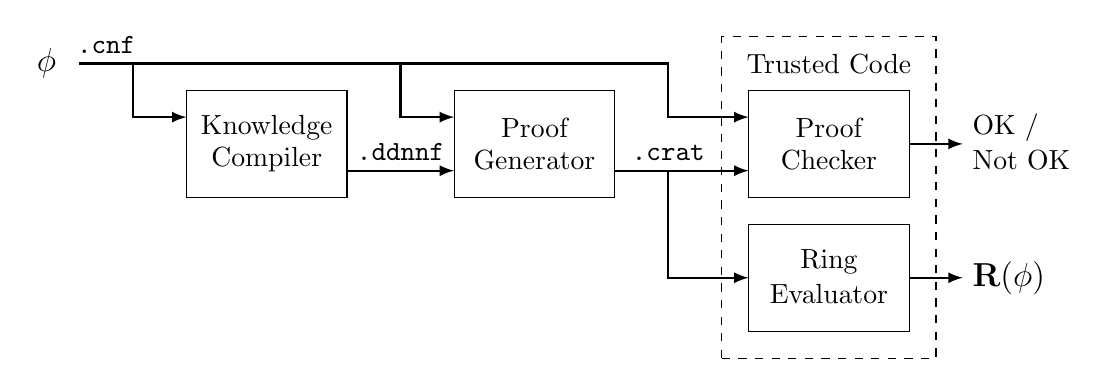
\begin{tikzpicture}[scale=0.17]
  \draw (8,10) rectangle (20,18);
  \node at (14,15.2) {Knowledge};
  \node at (14,12.8) {Compiler};

  \draw (28,10) rectangle (40,18);
  \node at (34,15.2) {Proof};
  \node at (34,12.8) {Generator};


  \draw (50,10) rectangle (62,18);
  \node at (56,15.2) {Proof};
  \node at (56,12.8) {Checker};

  \draw (50,0) rectangle (62,8);
  \node at (56,5.2) {Ring};
  \node at (56,2.8) {Evaluator};

  \draw[dashed] (48,-2) rectangle (64,22);
  \node at (56,20) {Trusted Code};

  %% CNF
  \draw[thick] (0,20) -- (44,20) -- (44,16) [-latex] -- (50,16);
  \draw[thick] (4,20) -- (4,16) [-latex] -- (8,16);
  \draw[thick] (24,20) -- (24,16) [-latex] -- (28,16);
  \node [left] at (-1,20) {\large {$\phi$}};
  \node [above] at (2,20) {\texttt{.cnf}};

  %% NNF
  \draw[thick] (20,12) [-latex] -- (28,12);
  \node [above] at (24,12) {\texttt{.ddnnf}};

  %% CRAT
  \draw[thick] (40,12) [-latex] -- (50,12);
  \draw[thick] (44,12) -- (44,4) [-latex] -- (50,4);
  \node [above] at (44,12) {\texttt{.crat}};

  %% OK/Not
  \draw[thick] (62,14) [-latex] -- (66,14) ;
  \node [right] at (66,15.2) { OK /} ;
  \node [right] at (66,12.8) { Not OK} ;
  \draw[thick] (62,4) [-latex] -- (66,4) ;
  \node [right] at (66,4) {\large {$\textbf{R}(\phi)$}};

\end{tikzpicture}
}
\caption{Certifying toolchain.
  The output of a standard knowledge compiler is converted into a combined graph/proof (CRAT)
  which can be independently checked and evaluated}
\label{fig:chain}
\end{figure}


Figure~\ref{fig:chain} illustrates our certifying knowledge compilation
and (weighted) model counting toolchain.  A
{\em proof generator} generates a CRAT description from a d-DNNF
graph produced by \dfour{}, a state-of-the-art knowledge compiler.
A {\em proof checker} then verifies that the combination of CNF and CRAT files
satisfy our rules, and a {\em ring evaluator} can compute
either a standard or weighted model count from the POG\@ representation.
We evaluate the capabilities of this toolchain using
benchmark formulas from the 2022 standard and weighted model
competitions.  Our tools are able to handle all but the largest d-DNNF
graphs generated by \dfour{}.
As the dashed box in Figure~\ref{fig:chain} indicates, this toolchain
moves the root of trust away from the complex and highly
optimized knowledge compiler to a relatively simple checker and
evaluator.  Importantly, the proof generator need not be
trusted---its errors will be caught by the proof checker.

To ensure soundness of the abstract CRAT proof system, as well as correctness of its
concrete implementation, we formally verified the proof system as well as versions
of the proof checker and ring evaluator in the \lean{} proof assistant~\cite{demoura:cade:2021}.
Running these two programs on a particular CRAT file gives assurance that the proof
and the model count are correct. Our experience with developing a formally verified
proof checker has shown that, even within the well-understood framework of extended
resolution, it can be challenging to formulate a full set of requirements that guarantee soundness.
In fact, subtle details in the partitioned sum rule were identified during this process.

\section{Related Work}

Generating proofs of unsatisfiability in SAT solvers has a long
tradition~\cite{ZhangMalik} and has become widely accepted due to the
formulation of clausal proof systems for which proofs can readily be
generated and efficiently (and, in some cases, formally) checked
\cite{cruz-cade-2017,RAT,Tan:2021,wetzler14_drattrim}.  Some progress
has also been made on extending these proof systems to other domains,
including quantified Boolean
formulas~\cite{bryant:cade:2021,heule:JAR2014}.

Fichte, Hecher, and Roland~\cite{fichte:sat:2022} devised the MICE
proof framework for model counting programs.  Their proof rules are
based on the algorithmic steps commonly used by model counting
programs, and they present a series of lemmas and a theorem stating
that their checking framework is sound.  They also present
experimental results for cases where they modify existing model
counters to generate proof traces, and where they generate proof
traces from d-DNNF graphs.
%% They have not formally verified their
%%proof framework or created a formally verified checker.

Our toolchain is not directly comparable to theirs---they directly
certify the numeric value produced by a model counter, while we 
certify that the graph generated by a knowledge compiler is logically
equivalent to the input formula.  We can also validate the unweighted or
weighted count generated from that representation.
%% Their tool
%% chain can be applied to some programs that are pure model counters,
%%while ours can be applied to pure knowledge compilers.
Nonetheless,
we compare the performance of our toolchain to theirs as part of our
experimental evaluation in Appendix~\ref{app:experiments}.

We know of no other
work addressing the question of certifying the output of a knowledge
compiler.

\section{Logical Foundations}
\label{section:logical:foundations}

  Let $\varset$ denote a set of Boolean variables, and let $\assign$
  be an {\em assignment} of truth values to some subset of the
  variables, where $0$ denotes false and $1$ denotes true, i.e.,
  $\assign \colon \varset' \rightarrow \{0,1\}$ for some $\varset'
  \subseteq \varset$.  We say the assignment is {\em total} when it
  assigns a value to every variable ($\varset' = \varset$), and that
  it is {\em partial} otherwise.
  The set of all possible total assignments over
  $\varset$ is denoted $\uassign$.

For each variable $x \in \varset$,
  we define the {\em literals} $x$ and $\obar{x}$, where $\obar{x}$ is the
  negation of $x$. An
  assignment $\assign$ can be viewed as a set of literals, where
  we write $\lit \in \assign$ when $\lit = x$ and $\assign(x) = 1$ or when
  $\lit = \obar{x}$ and $\assign(x) = 0$.  We write the negation of literal $\lit$ as $\obar{\lit}$.  That is, $\obar{\lit} = \obar{x}$ when $\lit = x$ and
$\obar{\lit} = x$ when $\lit = \obar{x}$.


\begin{definition}[Boolean Formulas]
  The set of Boolean formulas is defined recursively.  Each
  formula $\phi$ has an associated {\em dependency set}
  $\dependencyset(\phi)  \subseteq \varset$, and a set of models $\modelset(\phi)$,
  consisting of total assignments that satisfy the formula:
  \begin{enumerate}
  \item Boolean constants $0$ and $1$ are Boolean formulas,
    with $\dependencyset(0) = \dependencyset(1) = \emptyset$, with $\modelset(0) = \emptyset$, and with $\modelset(1) = \uassign$.
  \item Variable $x$ is a Boolean formula, with $\dependencyset(x) = \{x\}$
    and $\modelset(x) = \{\assign \in \uassign | \assign(x)=1\}$.
  \item For formula $\phi$, its {\em negation}, written $\boolnot \phi$ is a Boolean formula,
    with $\dependencyset(\boolnot \phi) = \dependencyset(\phi)$ and $\modelset(\boolnot \phi) = \uassign - \modelset(\phi)$.
  \item For formulas $\phi_1, \phi_2, \ldots, \phi_k$, their {\em product} $\phi = \bigwedge_{i=1 \leq i \leq k} \phi_i$ is a Boolean formula, with
      $\dependencyset(\phi) = \bigcup_{i=1 \leq i \leq k} \dependencyset(\phi_i)$ and
      $\modelset(\phi) = \bigcap_{i=1 \leq i \leq k} \modelset(\phi_i)$.
  \item For formulas $\phi_1, \phi_2, \ldots, \phi_k$, their {\em sum} $\phi = \bigvee_{i=1 \leq i \leq k} \phi_i$ is a Boolean formula, with
      $\dependencyset(\phi) = \bigcup_{i=1 \leq i \leq k} \dependencyset(\phi_i)$ and
      $\modelset(\phi) = \bigcup_{i=1 \leq i \leq k} \modelset(\phi_i)$.
  \end{enumerate}
\label{def:boolean}
\end{definition}


  We highlight two special classes of Boolean formulas.  A formula is
  in {\em negation normal form} when negation is applied only to variables.  A
  formula is in {\em conjunctive normal form} (CNF) when 1) it is in
  negation normal form, and 2) sum is applied only to literals.  A CNF
  formula can be represented as a set of {\em clauses}, each of which is a
  set of literals.  Each clause represents the sum of the
  literals, and the formula is the product of its clauses.  We use
  set notation to reference the clauses within a formula and the
  literals within a clause.  A clause consisting of a single literal is referred to as a {\em unit} clause and the literal as a {\em unit} literal.
This literal must be assigned value $1$ by any satisfying assignment of the formula.

\begin{definition}[Partitioned-Operation Formula]
  A {\em partitioned-operation formula}
 satisfies the following for all product and sum operations:
      \begin{enumerate}
      \item The arguments to each product must have disjoint dependency sets.  That is, operation
        $\bigwedge_{i=1 \leq i \leq k} \phi_i$ requires $\dependencyset(\phi_i) \cap \dependencyset(\phi_j) = \emptyset$ for $1 \leq i < j \leq k$.
      \item The arguments to each sum must have disjoint models.  That is, operation
        $\bigvee_{i=1 \leq i \leq k} \phi_i$ requires $\modelset(\phi_i) \cap \modelset(\phi_j) = \emptyset$ for $1 \leq i < j \leq k$.
      \end{enumerate}
\end{definition}
     We let $\pand$ and $\por$ denote the product and sum operations in a partitioned-operation formula.

  \section{Ring Evaluation of a Boolean Formula}

We propose a general framework for summarizing properties of Boolean
formulas along the lines of algebraic model counting~\cite{kimmig:jal:2017}.

\begin{definition}[Commutative Ring]
  A {\em commutative ring} $\ring$ is an algebraic structure
  $\langle \dset, \radd, \rmul, \addident, \mulident \rangle$,
  with elements in the set $\dset$ and with commutative and
  associative operations $\radd$ (addition) and $\rmul$ (multiplication),
  such that multiplication distributes
  over addition.  $\addident$ is the additive identity and $\mulident$ is
  the multiplicative identity.  Every element $a \in \dset$ has an
  {\em additive inverse} $-a$ such that $a + -a = \addident$.
\label{def:ring}
\end{definition}
We write $a - b$ as a shorthand for $a + -b$.

\begin{definition}[Ring Evaluation Problem]
\label{def:ring_evaluation}
  For commutative ring $\ring$, a {\em ring weight function} associates a value $w(x) \in \dset$ with
  every variable $x \in \varset$.  We then define $w(\obar{x})$ to equal $\mulident-w(x)$.

  For Boolean formula $\phi$, and ring weight function $w$, the {\em ring evaluation problem} is to compute:
  \begin{eqnarray}
    \rep(\phi, w) & = & \sum_{\alpha \in \modelset(\phi)} \;\; \prod_{\lit \in \alpha} w(\ell) \label{eqn:rep}
  \end{eqnarray}
  In this equation, sum \scalebox{0.8}{$\sum$} is computed using addition operation $\radd$, and product \scalebox{0.8}{$\prod$} is computed using multiplication operation $\rmul$.
\label{def:weight}
\end{definition}

Many important properties of Boolean formulas can be
expressed as ring evaluation problems.  The
{\em model counting} problem for formula $\phi$ requires determining $|\modelset(\phi)|$.
It can be cast as a ring evaluation problem by having $\radd$ and
$\rmul$ be addition and multiplication over rational numbers and using
weight function $w(x) = 1/2$ for every variable $x$.
Ring evaluation of formula $\phi$ gives the {\em density} of
the formula, i.e., the fraction of all possible total assignments that are
models.  For $n = |\varset|$, scaling the density by $2^n$
yields the number of models.  This formulation avoids the need for a ``smoothing'' operation,
in which redundant expressions are inserted into the formula~\cite{darwiche:jair:2002}.

The {\em weighted model counting}  problem is also defined over
rational numbers.  Some formulations  allow
independently assigning weights $W(x)$ and $W(\obar{x})$ for each variable $x$ and its complement, with the possibility that
$W(x) + W(\obar{x}) \not = 1$.
We can cast this as a
ring evaluation problem by letting $r(x) = W(x) + W(\obar{x})$,
performing ring evaluation with weight function $w(x) = W(x)/r(x)$ for each
variable $x$, and computing the weighted count
as $\rep(\phi, w)\; \rmul\; \prod_{x \in \varset} r(x)$.
Of course, this requires that $r(x) \not = 0$ for all $x \in \varset$.

The {\em function hashing problem} provides a test
of inequivalence for Boolean formulas.  That is, for $n = |\varset|$, let $\ring$ be a
finite  field with $|\dset| = m$ such that $m \geq 2 n$.  For each $x \in \varset$, chose a value from $\dset$ at random for $w(x)$.  Two formulas
$\phi_1$ and $\phi_2$ will clearly have $\rep(\phi_1, w) = \rep(\phi_2, w)$
if they are logically equivalent.
%, and if $\rep(\phi_1, w) \not = \rep(\phi_2, w)$, then they are clearly inequivalent.
If they are not equivalent, then
the probability that $\rep(\phi_1, w) \not = \rep(\phi_2, w)$ will be at
least $\left(1-\frac{1}{m}\right)^n \geq \left(1-\frac{1}{2n}\right)^n > 1/2$.
Function hashing can therefore be used as part of a
randomized algorithm for equivalence testing~\cite{blum:ipl:1980}.

%We compare ring evaluation to algebraic model counting in Section~\ref{sect:future}.

\section{Partitioned-Operation Graphs (POGs)}
\label{sect:pog}

Performing ring evaluation on an arbitrary Boolean formula could be intractable, but it is straightforward for a formula with partitioned operations:
\begin{proposition}
\label{prop:ring:eval}
Ring evaluation with operations $\boolnot$, $\pand$, and $\por$ satisfies the following for any weight function $w$:
\begin{eqnarray}
%% V1
\textstyle
\rep(\boolnot \phi,\; w) &=& \mulident - \rep(\phi, w) \label{eqn:ring:negation} \\
\textstyle
\scalebox{1.2}{\rep}\left(\Pand_{i=1 \leq i \leq k} \phi_i,\; w \right) &=& \prod_{i=1 \leq i \leq k} \rep(\phi_i, w) \label{eqn:ring:product} \\
\textstyle
\scalebox{1.2}{\rep}\left(\Por_{i=1 \leq i \leq k} \phi_i,\; w\right) &=& \sum_{i=1 \leq i \leq k} \rep(\phi_i, w) \label{eqn:ring:sum}
%% V2
%\rep(\boolnot \phi, w) &=& \mulident - \rep(\phi, w) \label{eqn:ring:negation} \\
%\rep\left(\phi_1, w \pand \dots \pand \phi_k, w \right) &=& \prod_{i=1..k} \rep(\phi_i, w) \label{eqn:ring:product} \\
%\rep\left(\phi_1, w \por \dots \por \phi_k, w \right) &=& \sum_{i=1..k} \rep(\phi_i, w) \label{eqn:ring:sum}
%\rep\left(\Pand_{i=1 \leq i \leq k} \phi_i, w \right) &=& \prod_{i=1 \leq i \leq k} \rep(\phi_i, w) \label{eqn:ring:product} \\
%\rep\left(\Por_{i=1 \leq i \leq k} \phi_i, w\right) &=& \sum_{i=1 \leq i \leq k} \rep(\phi_i, w) \label{eqn:ring:sum}
\end{eqnarray}
\end{proposition}
As is described in Section~\ref{subsection:counting}, we have proved these three equations using \lean{}.

A {\em partitioned-operation graph} (POG) is a directed, acyclic graph
with nodes $N$ and edges $E \subseteq N \times N$.  We denote nodes with boldface symbols, such as $\nodeu$ and $\nodev$.
When $(\nodeu,\nodev) \in E$,
node $\nodev$ is said to be a {\em child} of node $\nodeu$.
The in- and out-degrees of node $\nodeu$ are defined as $\indegree(\nodeu) = | E \cap (N \times \{\nodeu\}) |$, and
$\outdegree(\nodeu) = | E \cap (\{\nodeu\} \times N) |$.
Node $\nodeu$ is said to be {\em terminal} if $\outdegree(\nodeu) = 0$.  A terminal node is labeled by a Boolean constant or variable.
Node $\nodeu$ is said to be {\em nonterminal} if $\outdegree(\nodeu) > 0$.
A nonterminal node is labeled by one of the three Boolean operations: $\boolnot$, $\pand$ or $\por$.
Node $\nodeu$ can be labeled with $\boolnot$ only if $\outdegree(\nodeu) = 1$.
It can be labeled with operation $\pand$ or $\por$ only if it satisfies the partitioning restriction for that operation.
There is a unique {\em root node} $\noder$ such that $\indegree(\noder) = 0$.

In essence, a POG represents a partitioned-operation
formula with a sharing of common subformulas.  Indeed, every node in the graph can be viewed as a partitioned-operation formula, and so we write
$\phi_{\nodeu}$ as the formula denoted by node $\nodeu$.
Each such formula has a set of models, and we write $\modelset(\nodeu)$ as a shorthand for $\modelset(\phi_{\nodeu})$.

We define the {\em size} of POG $P$, written $|P|$, to be the
the number of nodes labeled $\pand$ or $\por$ plus the number of edges from these nodes to their children.  Ring
evaluation of $P$ can be performed with at most $|P|$ ring
operations by traversing the graph from the terminal nodes up to
the root, computing a value $\rep(\nodeu, w)$ for each node $\nodeu$.
The final result is then $\rep(\noder, w)$.

POGs generalize the d-DNNF graphs in two ways:
\begin{itemize}
\item They allow negation of arbitrary nodes in the graph, not just
  variables.
  %, and so we allow it in the interest of generality.
%%  Negation could be useful in some contexts, such as when
%%  converting binary decision diagrams (BDDs) having complemented
%%  edges~\cite{brace-dac-1990,minato-dac-1990} into POGs.
\item They allow arbitrary arguments to a $\por$ operation, as long as
  these have disjoint models.  By contrast, each
  sum node $\nodeu$ in a d-DNNF must have two children $\nodeu_1$ and $\nodeu_0$, and for these there must be a {\em decision variable} $x$ such that
  any total assignment $\assign \in  \modelset(\nodeu_b)$ has $\assign(x)=b$, for $b \in \{0,1\}$.
%%Our generalization is provided to allow an
%%  encoding of Sentential Decision Diagrams (SDDs)~\cite{darwiche:ijcai:2011} as
%%  POGs.  This is discussed in Section~\ref{sect:future}, describing possible future research.
\end{itemize}
  These generalizations allow more flexibility in the POG
  representation while maintaining the ability to efficiently perform ring evaluation.

\section{Clausal Proof Frameworks}

A proof in our framework takes the form of a sequence of clause addition
and deletion steps, with each step preserving the set of solutions to
the original formula.
The status of the proof at any step is represented as
a set of {\em active} clauses $\phi$, i.e., those that
have been added but not yet deleted.
Our framework is based
on {\em extended} resolution~\cite{Tseitin:1983}, where proof
steps can introduce new {\em extension variables} encoding Boolean formulas over input and prior extension variables.
Let $Z$
denote the set of extension variables occuring in formula $\phi$.
Starting with input formula $\inputformula$,
the proof must maintain the invariant that
$\inputformula \ifandonlyif \exists Z\,\phi$.

Clauses can be added in two different ways.  One is when they serve as
the {\em defining clauses} for an extension variable.  This form
occurs only when defining $\pand$ and $\por$ operations, as is
described in Section~\ref{sect:crat}.  Clauses can also be added or
deleted based on {\em implication redundancy}.  That is, when clause
$C$ satisfies $\phi \imply C$ for formula $\phi$, then it can either
be added to $\phi$ to create the formula $\phi \cup \{C\}$ or it can be deleted
from $\phi \cup \{C\}$ to create $\phi$.

We use {\em reverse unit propagation} (RUP) to certify
implication redundancy when adding or deleting
clauses~\cite{goldberg,vangelder08_verifying_rup_proofs}.
RUP
is the core rule supported by standard
proof checkers~\cite{RAT,wetzler14_drattrim} for propositional logic. It provides a simple and efficient
way to check a sequence of applications of the resolution proof rule~\cite{robinson-1965}.
Let $C = \{\lit_1, \lit_2, \ldots,\lit_p\}$ be a clause to be
proved redundant with respect to formula $\phi$.  Let $D_1, D_2, \ldots, D_k$ be a sequence of supporting
{\em antecedent} clauses, such that each $D_i$ is in $\phi$.
A RUP step
proves that $\bigwedge_{1\leq i \leq k} D_i \imply C$ by showing
that the combination of the antecedents plus the negation of $C$ leads
to a contradiction.  The negation of $C$ is the formula
$\overline{\lit}_1 \land \overline{\lit}_2 \land \cdots \land
\overline{\lit}_p$, having a CNF representation consisting of $p$ unit
clauses of the form $\obar{\lit}_i$ for $1 \leq i \leq p$.  A RUP
check processes the clauses of the antecedent in sequence, inferring
additional unit clauses.  In processing clause $D_i$, if all but one
of the literals in the clause is the negation of one of the
accumulated unit clauses, then we can add this literal to the
accumulated set.  That is, all but this literal have been falsified,
and so it must be set to true for the clause to be satisfied.  The
final step with clause $D_k$ must cause a contradiction, i.e., all of
its literals are falsified by the accumulated unit clauses.

Compared to the proofs of unsatisfiability generated by SAT solvers,
ours have important differences.  Most
significantly, each proof step must preserve the set of solutions with respect to the input variables.
By contrast, an unsatisfiability proof need only guarantee that
no proof step cause a satisfiable set of clauses to become
unsatisfiable.  As a consequence, our proofs must justify clause deletions as well as clause additions.


\section{The CRAT POG Representation and Proof System}
\label{sect:crat}


%% The proof system is based on extended
%% resolution~\cite{Tseitin:1983} with reverse unit propagation
%% (RUP)~\cite{goldberg,vangelder08_verifying_rup_proofs} as the core method for
%% proving that a set of clauses logically implies another clause.
%% Alternate version
%% knowledge compilation.  The proof system is based on extended
%% resolution~\cite{Tseitin:1983} with reverse unit propagation
%% (RUP)~\cite{goldberg,vangelder08_verifying_rup_proofs} as the core method for
%% proving that a set of clauses logically implies another clause.
%%
%% As an example, consider the formula $\varphi = (\obar{a} \lor b) \land (\obar{b} \lor c \lor \obar{e}) \land (\obar c \lor d)$
%% and a RUP step to derive the target clause $(\obar{a} \lor d \lor \obar{e})$ from the three clauses from $\varphi$.
%% A RUP proof would take the following form.  We start with the assignment that falsifies the target clause. This assignment
%% is extended by clauses in $\varphi$ that become unit and eventually the empty clause. In the illustration below, the
%% involved clauses (antecedents) are shown in the order that they became unit / falsified.
%%
%% \begin{center}
%%   \begin{tabular}{lcccc}
%%          & \makebox[15mm]{Target}    & \makebox[10mm]{} & \makebox[10mm]{Antecedents} & \makebox[10mm]{} \\
%%   Clause & $\obar{a} \lor d \lor \obar{e}$ & $\obar{c} \lor d$  & $\obar{e} \lor \obar{b} \lor c$   & $\obar{a} \lor b$ \\
%%   \midrule
%%   Units  & $a$, $\obar{d}$, $e$      &  $\obar{c}$             & $\obar{b}$                         & $\nil$ \\
%%   \end{tabular}
%% \end{center}
%%
%% RUP is an alternative formulation of resolution.  For target clause
%% $C$, it can be seen that applying resolution operations to the
%% antecedent clauses from right to left will derive a clause $C'$ such
%% that $C' \subseteq C$.  By {\em subsumption} %~\cite{philipp:lpar:2017},
%% we then have $C' \rightarrow C$.  Compared to listing each resolution
%% operation as a separate step, using RUP as the basic proof step makes
%% the proofs more compact.
%%
%% As is shown in Figure~\ref{fig:chain}
%% two programs are involved in producing a certified compilation of a formula:
%% \begin{itemize}
%% \item The {\em proof generator} produces a CRAT file that both defines the POG and gives a proof that the POG is logically equivalent to the input formula.
%% As the figure indicates, the generator starts with the output of another knowledge compiler, such as one generating a d-DNNF representation of the formula.
%% \item The {\em proof checker} ensures that all of the proof conditions are satisfied.
%% \end{itemize}
%% >>>>>>> 9c1793da858d00e5d4022d6d33c009848ba2083b

A CRAT file provides both a declaration of a POG, as well as a checkable
proof that a Boolean formula, given in conjunctive normal
form, is logically equivalent to the POG\@.
The proof format draws its inspiration from the LRAT~\cite{lrat} and
QRAT~\cite{heule:JAR2014} formats for unquantified and quantified Boolean formulas, respectively.
Key properties include:
\begin{itemize}
  \item
  The file contains declarations of $\pand$ and $\por$ operations to describe the POG.
  Declaring a node $\nodeu$
implicitly adds an {\em extension} variable $u$ and a set of {\em defining} clauses $\theta_{u}$
  encoding the product or sum operation.
%  This is the only means for adding extension variables to the proof.
\item Boolean negation is supported implicitly by allowing the
  arguments of the $\por$ and $\pand$ operations to be literals and not just
  variables.
\item
  The file contains explicit clause addition steps.
  A clause can only be added if it is logically implied by the existing clauses.
  A sequence of clause identifiers must be listed as a {\em hint} providing a RUP verification of the implication.
\item
  The file contains explicit clause deletion steps.
  A clause can only be deleted if it is logically implied by the remaining clauses.
  A sequence of clause identifiers must be listed as a {\em hint} providing a RUP verification of the implication.
\item The checker must track the dependency set for every input and
  extension variable.  For each $\pand$ operation, the checker must ensure that the dependency sets for its arguments are disjoint.
  The associated extension variable has a dependency set equal to the union of those of its arguments.
\item Declaring a $\por$ operation requires a sequence of clauses
  providing a RUP proof that the arguments are mutually exclusive.
  Only binary $\por$ operations are allowed to avoid requiring multiple proofs of disjointness
%  Generalizing to $k$ arguments would require
%  $k\,(k-1)/2$ proofs of disjointness.
\end{itemize}

\subsection{Syntax}
\label{subsection:syntax}

\begin{table}
  \caption{CRAT Step Types.  $C$: clause identifier, $L$: literal, $V$: variable}
  \label{tab:crat:syntax}
\centering{
  \begin{tabular}{lllll}
    \toprule
    \multicolumn{4}{c}{Rule} & \multicolumn{1}{c}{Description} \\
    \midrule
    \makebox[5mm][l]{$C$} & \makebox[10mm][l]{\tt a}  & \makebox[15mm][l]{$L^{*}$ {\tt 0}} & \makebox[15mm][l]{$C^{+}$ {\tt 0}}  & \makebox[20mm][l]{Add RUP clause} \\
     & {\tt d} & $C$             & $C^{+}$  {\tt 0} & Delete RUP clause \\
    \midrule
    $C$    & {\tt p} & $V \; L^{*}$ {\tt 0}    &                  & Declare $\pand$ operation \\
    $C$    & {\tt s} & $V \; L \; L$    & $C^{+}$ {\tt 0}  & Declare $\por$ operation \\
    \midrule
     & {\tt r} & $L$             &            & Declare root literal\\
    \bottomrule
  \end{tabular}
  }
\end{table}

Table~\ref{tab:crat:syntax} shows the declarations that can occur in a CRAT file.
%% The checker is provided with the input formula as a separate file.
As with other clausal proof formats, a variable is
represented by a positive integer $v$, with the first ones being input
variables and successive ones being extension variables.  Literal $\lit$
is represented by a signed integer, with $-v$ being the logical negation of
variable $v$.  Each clause is indicated by a positive integer
identifier $C$, with the first ones being the IDs of the input clauses and successive
ones being the IDs of added clauses.  Clause identifiers must be totally ordered,
such that any clause identifier $C'$ given in the hint when adding clause $C$ must have $C' < C$.

The first set of proof rules are similar to those in other clausal
proofs.
Clauses can be added via RUP addition
(command {\tt a}), with a sequence of antecedent clauses (the
``hint'').
Similarly for clause deletion (command {\tt d}).

\begin{table}
\caption{Defining Clauses for Product (A) and Sum (B) Operations}
\begin{minipage}{0.54\textwidth}
\begin{center}
\begin{tabular}{cccccc}
\multicolumn{6}{c}{(A).  Product Operation $\pand$}\\
\toprule
\makebox[10mm]{ID} & \multicolumn{5}{c}{Clause} \\
\midrule
  $i$ & $v$ & $-\lit_1$ & $-\lit_2$ & $\cdots$ & $-\lit_k$\\
  $i\!+\!1$ & $-v$ & $\lit_1$  \\
  $i\!+\!2$ & $-v$ & $\lit_2$  \\
  & $\ldots$ \\
  $i\!+\!k$ & $-v$ & $\lit_k$  \\
\bottomrule
\end{tabular}
\end{center}
\end{minipage}
\begin{minipage}{0.44\textwidth}
\begin{center}
\begin{tabular}{cccc}
\multicolumn{4}{c}{(B).  Sum Operation $\por$}\\
\toprule
\makebox[10mm]{ID} & \multicolumn{3}{c}{Clause} \\
\midrule
  $i$ & $-v$ & $\lit_1$ & $\lit_2$ \\
  $i\!+\!1$ & $v$ & $-\lit_1$ \\
  $i\!+\!2$ & $v$ & $-\lit_2$ \\
\bottomrule
$\;$ \\
$\;$ \\
\end{tabular}
\end{center}
\end{minipage}
\label{tab:defining}
\end{table}

The declaration of a {\em product} operation, creating a node with operation $\pand$,
 has the form:
\begin{center}
\begin{tabular}{ccccccccc}
  \makebox[5mm]{$i$} & \makebox[5mm]{{\tt p}} & \makebox[5mm]{$v$} & \makebox[5mm]{$\lit_1$} & \makebox[5mm]{$\lit_2$} &
  \makebox[5mm]{$\cdots$} & \makebox[5mm]{$\lit_k$} & \makebox[5mm]{\tt 0} \\
\end{tabular}
\end{center}
Integer $i$ is a new clause ID, $v$ is a positive integer that does not
correspond to any previous variable, and $\lit_1, \lit_2, \ldots, \lit_k$ is a sequence of $k$
integers representing literals of existing variables.
As Table~\ref{tab:defining}(A) shows,
this declaration implicitly causes $k+1$ clauses to be added to the proof, defining extension variable $v$ to be the product of its arguments.

The dependency sets for the arguments represented by each pair of
literals $\lit_i$
and $\lit_{j}$ must
be disjoint, for $1 \leq i < j \leq k$.  A product operation may have no arguments,
representing Boolean constant $1$.  The only clause added to the proof will be
the unit literal $v$.  A reference to literal $-v$ then provides a way
of representing constant $0$.

The declaration of a {\em sum} operation, creating a node with operation $\por$, has the form:
\begin{center}
\begin{tabular}{ccccccc}
  \makebox[5mm]{$i$} & \makebox[5mm]{{\tt s}} & \makebox[5mm]{$v$} & \makebox[5mm]{$\lit_1$} & \makebox[5mm]{$\lit_2$}
\makebox[5mm]{$H$} & \makebox[5mm]{$\texttt{0}$} \\
\end{tabular}
\end{center}
Integer $i$ is a new clause ID, $v$ is a positive integer that does
not correspond to any previous variable, and $\lit_1$ and $\lit_2$ are
signed integers representing literals of existing variables.  Hint $H$
consists of a
sequence of clause IDs, all of which must be defining clauses for other POG operations.
As Table~\ref{tab:defining}(B) shows,
this declaration implicitly causes three clauses to be added to the proof, defining extension variable $v$ to be the sum of its arguments.
The hint must provide a RUP proof of the clause $\obar{\lit}_1 \lor \obar{\lit}_2$, showing that the two children of this node have disjoint models.

Finally, the literal denoting the root of the POG is declared with the
{\tt r} command.  It can occur anywhere in the file.  Except in degenerate cases, it
will be the extension variable representing the root of a graph.
%, but in
%degenerate cases it can be the positive or negative literal of an
%input variable.

\subsection{Semantics}

The defining clauses for a product or sum
operation uniquely define the value of its extension variable for any assignment of values to the argument variables.
For the
extension variable $u$ associated with any POG node $\nodeu$, we can therefore
assume that any total assignment $\assign$ to the input variables will
also assign a value to $u$ such that $\assign(u) =
1$ if and only if $\assign \in \modelset(\nodeu)$.  For a POG with
root literal $r$, we can define its set of models $\modelset(P)$ as
the set of all total assignments $\assign$ such that $\assign(r) = 1$.

%% A CRAT proof follows the same general form as a QRAT dual
%% proof~\cite{bryant:cade:2021}---one that ensures that each clause
%% addition and each clause deletion preserves equivalence.  With CRAT,
%% however, clauses are defined both explicitly and implicitly.  Starting
%% with the set of input clauses, the proof consists of a sequence of
%% steps that both add and delete clauses.  Each addition must be truth
%% preserving, that is, any satisfying total assignment for the set of clauses
%% before clause addition should still be a satisfying assignment afterwards.
%% Each deletion must be falsehood preserving.  That is, there can be no
%% new satisfying assignments when the clause is deleted.

The sequence of operator declarations, asserted clauses, and
clause deletions represents a systematic transformation of the input formula
into a POG formula.  Validating all of these steps serves to prove that the
POG is logically equivalent to the input formula.
At the completion of the proof, the following conditions must hold:
\begin{enumerate}
\item There is exactly one remaining clause that was added via RUP
  addition, and this is a unit clause consisting of root literal $r$.
\item All of the input clauses have been deleted.
\end{enumerate}
In other words, at the end of the proof it must hold that the active clauses be exactly those
in $\pogformula = \{\{r\}\} \cup \; \bigcup_{\nodeu \in P} \theta_{u}$, the formula consisting
of unit clause $r$ and the defining clauses of the POG nodes. We can write
$\modelset(P)$ as a shorthand for $\modelset(\pogformula)$, recognizing that
any assignment to the input variables implicitly defines the assignments to the extension variables.
Let $\inputformula$ denote the input formula.
The sequence of clause addition steps provides a {\em forward implication} proof that
$\modelset(\inputformula) \subseteq \modelset(P)$.  That is, any total
assignment $\assign$ satisfying the input formula must also satisfy
the formula represented by the POG\@.
Conversely,
each proof step that deletes an input clause proves that any
total assignment $\alpha$ that falsifies the clause must
assign $\assign(r) = 0$.  Deleting all but the final asserted clause and all input clauses provides a {\em reverse implication} proof
that
$\modelset(P) \subseteq \modelset(\inputformula)$.

Appendix~\ref{app:crat:example} shows the CRAT description for
an input formula with five clauses, yielding a POG with five
nonterminal nodes.  It explains how the clause addition and deletion
steps yield a proof of equivalence between the input formula and its POG
representation.

\section{Generating CRAT from d-DNNF}
\label{section:generating:crat}

%%Figure~\ref{fig:chain} illustrates one method of generating a CRAT
%%file from an input formula in conjunctive normal form.  Our toolchain
%%is based on the \dfour{} knowledge compiler~\cite{lagniez:ijcai:2017},
%%but it would also work for other tools that use a top-down search
%%strategy to generate a d-DNNF representation.
Converting a d-DNNF
graph into a POG is straightforward---each node in a d-DNNF graph can
be directly represented as a POG node, although
our program performs simplifications to
eliminate Boolean constants.
Except in degenerate cases,
%where the formula is unsatisfiable or a tautology,
we can therefore assume
that the POG does not contain any constant nodes.
In addition, negation is only
applied to variables, and so we can merge the negation operations into the terminal nodes,
viewing the POG as consisting
of {\em literal} nodes corresponding to input variables and their negations, along with
{\em nonterminal} nodes, which can be further classified as {\em product} nodes and {\em sum} nodes.

\subsection{Forward implication proof}

For input formula $\inputformula$ and its translation into a POG $P$
with root literal $r$, the most challenging part of the proof is to
show that $\modelset(\inputformula) \subseteq \modelset(P)$, i.e.,
that any total assignment $\alpha$ that is a model of $\inputformula$
will yield $\assign(r) = 1$, for root literal $r$.  This part of the
proof consists of a series of clause assertions leading to one adding
$r$ as a unit clause.  We have devised two methods of generating this
proof.  The {\em monolithic} approach makes just one call to a
proof-generating SAT solver and has it determine the relationship
between the two representations.  The {\em structural} approach
recursively traverses the POG, generating proof obligations at each
node encountered.  It too may require calls to a proof-generating SAT
solver.

As notation,
let $\psi$ be a subset of the clauses in $\inputformula$.
For partial assignment
$\passign$, the expression  $\simplify{\psi}{\passign}$ denotes the set of clauses $\gamma$
obtained from $\psi$ by: i) eliminating any
clause containing a literal $\lit$ such that $\passign(\lit) = 1$,
ii) for the remaining clauses eliminating those literals $\lit$ for
which $\passign(\lit) = 0$, and iii) eliminating any duplicate clauses.
In doing these simplifications, we also track the {\em provenance}
of each simplified clause $C$, i.e., which of the (possibly multiple) input clauses simplified to become $C$.
More formally, for $C \in \simplify{\psi}{\passign}$, we let $\prov_{\passign}(C, \psi)$ denote
those clauses $C' \in \psi$, such that
$C' \subseteq C \cup \bigcup_{\lit \in \passign} \obar{\lit}$.
We then extend the definition of $\prov$ to any simplified formula
$\gamma$ as $\prov_{\passign}(\gamma, \psi) = \bigcup_{C \in \gamma} \prov_{\passign}(C, \psi)$.

The monolithic approach
takes advantage of the clausal representations of
the input formula $\inputformula$ and the POG formula $\pogformula$.
It can
express the negation of $\pogformula$ as $\neg \pogformula = \bigcup_{\nodeu\in P} \simplify{\theta_{u}}{\{\obar{r}\}}$.
Forward implication
will hold
when $\inputformula \imply \pogformula$, or  equivalently,
that the formula $\inputformula \land \neg \pogformula$
is unsatisfiable, where the
conjunction can be expressed as the union
of the two sets of clauses.  The proof generator writes the clauses to a file and invokes a proof-generating SAT solver.
For each clause $C$ in the unsatisfiability proof, it adds clause $\{r\} \cup C$ to the CRAT proof, and so the empty clause in the proof becomes the unit clause $r$.
Our experimental results show
that this approach can be very effective and generates short proofs
for smaller problems, but it does not scale well enough for routine
use.


We describe the structural approach to proof generation as a recursive procedure
$\validate(\nodeu, \passign, \psi)$ taking as arguments POG
node $\nodeu$, partial assignment
$\passign$, and a set of clauses $\psi \subseteq \inputformula$.
The procedure adds a number of clauses to the proof, culminating with
the addition of the {\em target} clause:
$u \lor \bigvee_{\lit \in \passign} \obar{\lit}$, indicating
that $(\bigwedge_{\lit \in \passign} \lit) \imply u$, i.e.,
that any total
assignment $\assign$ such that $\passign \subseteq \assign$
will assign $\assign(u) = 1$.
The top-level call has $\nodeu = \noder$, $\passign = \emptyset$, and $\psi = \inputformula$.
The result will therefore be to add unit clause $r$ to the proof.
Here we present a correct, but somewhat inefficient formulation of
$\validate$.  We then refine it with some optimizations.

The recursive call $\validate(u, \passign, \psi)$ assumes that we have
traversed a path from the root node down to node $\nodeu$, with the
literals encountered in the product nodes forming the partial
assignment $\passign$.  The set of clauses $\psi$ can be a proper
subset of the input clauses $\inputformula$ when a product node has caused
a splitting into clauses containing disjoint variables.
The subgraph with root node $\nodeu$ should be a POG representation of the formula
$\simplify{\psi}{\passign}$.  Having the
routine add its target clause indicates that any total assignment
$\assign$ such that $\passign \subseteq \assign$ will yield $\alpha(u) = 1$.

The process for generating such a proof depends on the form of node $\nodeu$:
\begin{enumerate}
\item If $\nodeu$ is a literal $\lit'$, then the formula
  $\simplify{\psi}{\passign}$ must consist of the single unit clause
  $C = \{\lit'\}$, such that any $C' \in \prov_{\passign}(C, \psi)$ must have $C' \subseteq \{ \lit' \} \cup\, \bigcup_{\lit \in \passign} \obar{\lit}$.
  Any of these can
  serve as the target clause.
\item If $\nodeu$ is a sum node with children $\nodeu_1$ and $\nodeu_0$,
  then, since the node originated from a d-DNNF graph, there must be
  some variable $x$ such that either $\nodeu_1$ is a literal node for $x$ or $\nodeu_1$ is a
  product node containing a literal node for $x$ as a child.  In either case, we
  recursively call $\validate(\nodeu_1, \passign \cup \{ x \}, \psi)$.
  This will cause the addition of the target clause
  $u_1 \lor \obar{x} \lor \bigvee_{\lit \in \passign} \obar{\lit}$.
Similarly, either $\nodeu_0$ is a literal node for $\obar{x}$ or $\nodeu_0$ is a product node containing a literal node for $\obar{x}$ as
  a child.  In either case, we recursively call $\validate(\nodeu_0, \passign \cup \{ \obar{x} \}, \psi)$,
  causing the addition of the target clause
  $u_0 \lor x \lor \bigvee_{\lit \in \passign} \obar{\lit}$.
  These recursive results can be combined with the second and third defining clauses for $\nodeu$
(see Table~\ref{tab:defining}(B))
  to generate the target clause for $\nodeu$.
\item If $\nodeu$ is a product node, then we can divide its children
  into a set of literal nodes $L$ and a set of nonterminal nodes $\nodeu_1, \nodeu_2, \ldots, \nodeu_k$.
  \begin{enumerate}
    \item For each literal
  $\lit \in L$, we must prove that any total assignment $\alpha$, such that
  $\passign \subset \alpha$ has $\alpha(\lit) = 1$.  In some
  cases, this can be done by simple Boolean constraint propagation (BCP).
  In other cases, we must prove that the formula
  $\simplify{\psi}{\passign \cup \{\obar{\lit}\}}$ is unsatisfiable.  We
  do so by writing the formula to a file, invoking a proof-generating
  SAT solver, and then converting the generated unsatisfiability proof
  into a sequence of clause additions in the CRAT file.
\item For a single nonterminal child ($k = 1$), we recursively call
  $\validate \left(\nodeu_1, \passign \cup \bigcup_{\lit \in L} \lit, \psi\right)$.
\item For multiple nonterminal children ($k > 1$),
  it must be the case that the clauses in
  $\gamma = \simplify{\psi}{\passign}$ can be partitioned into $k$ subsets
  $\gamma_1, \gamma_2, \ldots, \gamma_k$ such that $\dependencyset(\gamma_i)
  \cap \dependencyset(\gamma_j) = \emptyset$ for $1 \leq i < j \leq k$,
  and we can match each node $\nodeu_i$ to subset $\gamma_i$ based on its
  literals.
  For each $i$ such that $1 \leq i \leq k$, let $\psi_i = \prov_{\passign}(\gamma_i, \psi)$, i.e., those input clauses in $\psi$ that, when simplified, became clause partition $\gamma_i$.
  We recursively call
  $\validate \left(\nodeu_i, \passign \cup \bigcup_{\lit \in L} \lit, \psi_i\right)$.
\end{enumerate}
  We then generate the target clause for node $\nodeu$,
creating the hint by combining the results from the BCP and SAT calls for
  the literals, the recursively computed target clauses, and all but
  the first defining clause for node $\nodeu$
(see Table~\ref{tab:defining}(A)).
\end{enumerate}
Most of these steps involve a polynomial number of
operations per recursive call, with the exception of those that call
a SAT solver to validate a literal.

\subsection{Reverse implication proof}

Completing the equivalence proof of input formula $\inputformula$ and its POG
representation with root literal $r$ requires showing that
$\modelset(P) \subseteq \modelset(\inputformula)$.  This is done in the
CRAT framework by first deleting all asserted clauses, except for the
final unit clause for root literal $r$, and then deleting all of the
input clauses.  Suppose at some point in this process that we want to
delete clause $C$ such that the remaining set of clauses will form the
CNF formula $\phi$.  Deleting $C$ requires proving that
$\phi \imply C$.


The asserted clauses can be deleted in reverse order, using the same
hints that were used in their original assertions.  By reversing the
order, those clauses that were used in the hint when a clause was
added will still remain when it is deleted.

Each input clause deletion can be done as a single RUP step.  The
proof generator constructs the hint sequence from the defining
clauses of the POG nodes via a single, bottom-up pass through the
graph.  The RUP deletion proof for input clause $C$ effectively proves that any
total assignment $\assign$ that does not satisfy $C$ will yield
$\assign(r) = 0$.  It starts with the set of literals
$\{ \obar{\lit} \mid \lit \in C\}$, describing the required condition for
assignment $\assign$ to falsify clause $C$.
It then
adds literals via unit propagation until a
conflict arises.    Unit literal $r$ gets
added right away, setting up a potential conflict.

Working upward through the graph, node $\nodeu$ is {\em marked} when
the collected set of literals force $u$ to evaluate to $0$.  When marking $\nodeu$, the
program adds $\obar{u}$ to the RUP literals and adds the appropriate
defining clause to the hint.  A literal node for
$\lit$ will be marked if $\lit \in C$, with no hint required.  If
product node $\nodeu$ has some child $\nodeu_i$ that is marked, then
$\nodeu$ is marked and clause $i+1$ from among its defining clauses (see Table~\ref{tab:defining}(A)) is
added to the hint.  Marking sum node $\nodeu$ requires that its two children are marked.
The first defining
clause for this node (see Table~\ref{tab:defining}(B)) will then be added as a hint.  At the very end, the program
(assuming the reverse implication holds) will attempt to mark root
node $\noder$, which would require $\assign(r) = 0$, yielding a
conflict.

It can be seen that the reverse implication proof will be polynomial in the size of the POG\@, because
each clause deletion requires a single RUP step having a hint with length
bounded by the number of POG nodes.

\section{Optimizations}

The performance of the structural proof generator for forward implication, both in its execution time and
the size of the proof generated, can be improved by two optimizations
described here.  A key feature is that they do not require any changes
to the proof framework---they build on the power of extended
resolution to create new logical structures.  They
involve declaring new product nodes to encode products of literals.
These nodes are not part of the POG
representation of the formula; they serve only to enable the forward
implication proof.  Here we summarize the two optimizations.
Appendix~\ref{app:optimizations} provides more details.

{\em Literal Grouping:} A single recursive step of $\validate$ can encounter product nodes
having many---tens or even hundreds---of literals as children.  The
earlier formulation of $\validate$ considers each literal $\lit \in L$
separately, calling a SAT solver for every literal that cannot be
validated with BCP\@.  Literal grouping handles
all of these literals together.  It defines product node $\nodev$
having the literals as children.  The goal then becomes to prove that
any total assignment must yield 1 for extension variable $v$.  Calling
a solver with $v$ set to 0 yields an unsatisfiability proof that can
be mapped back to a sequence of clause additions in the CRAT file validating
all of the literals.

{\em Lemmas:} Our formulation of $\validate$ requires each call at a
node $\nodeu$ to recursively validate all of its children.  This
effectively expands the graph into a tree, potentially requiring an
exponential number of recursive steps.  Instead, for each node
$\nodeu$ having $\indegree(u) > 1$, the program can define and
generate the proof of a {\em lemma} for $\nodeu$ when it is first reached by
a call to $\validate$ and then apply this lemma for this and
subsequent calls.  The lemma states that the POG with root node
$\nodeu$ satisfies forward implication for a formula
$\gamma_{\nodeu}$, where some of the clauses in this formula are
input clauses from $\inputformula$, but others are simplified
versions of input clauses.
The key idea is to introduce product nodes to encode (via DeMorgan's
Laws) the simplified clauses and have these serve as lemma arguments.

The combination of these two optimization guarantees that 1) each call
to $\validate$ for a product node will cause at most one invocation of
the SAT solver, and 2) each call to $\validate$ for any node $\nodeu$
will cause further recursive calls only once.  Our experimental
results (Appendix~\ref{app:experiments}) shows that these
optimizations yield substantial benefits.


\section{A Formally Verified CRAT Checker and POG Model Counter}

We have implemented the rightmost two components of Figure~\ref{fig:chain}, namely the
proof checker and both model and weighted model counters, in the \lean{} programming language
and proof assistant~\cite{demoura:cade:2021}.
In this section, we briefly describe the functions we have implemented in Lean and
the specifications we have proved.
More information is provided in the Appendix~\ref{appendix:lean}.

\subsection{The Proof Checker}
\label{subsection:proof:checker}

Our specifications are built on a generic library for the syntax and semantics of
propositional logic. We define the data type \lstinline{PropForm Var} of propositional
formulas with variables \lstinline{Var}, which are positive natural numbers,
corresponding to the indexing of variables in the CNF file.
It is convenient to take a truth assignment \lstinline{PropAssignment Var} to a function that
assigns a Boolean value to every assignment, and later restrict attention to subsets of the
variables.

We define the following representations for CNF formulas.
A literal is represented as a nonzero integer, a clause is an array of literals,
and a CNF formula is an array of clauses.
\begin{lstlisting}
def ILit := { i : Int // i ≠ 0 }
abbrev IClause := Array ILit
abbrev ICnf := Array IClause
\end{lstlisting}
We also define functions \lstinline{ILit.toPropForm}, \lstinline{IClause.toPropForm},
and \lstinline{ICnf.toPropForm} to relate these to propositional formulas and their
semantics.

The goal of the proof checker is to construct a POG that is equivalent to the input CNF.
Each element of a POG  is either a variable, a binary disjunction,
or an arbitrary conjunction:
\begin{lstlisting}
inductive PogElt where
  | var  : Var → PogElt
  | disj : Var → ILit → ILit → PogElt
  | conj : Var → Array ILit → PogElt
\end{lstlisting}
In the first case, the argument \lstinline{x} in the expression
\lstinline{var x} is the index
of the variable; in \lstinline{disj x left right} and \lstinline{conj x args}
it is the definition number in the CRAT file. Note that representing edges as literals allows us to negate the arguments to \lstinline{disj} and \lstinline{conj}.
A \lstinline{Pog} is then simply an array of \lstinline{PogElt}.
For each POG \lstinline{P} and literal \lstinline{l}, we define
\lstinline{P.toPropForm l} to be the
propositional formula that arises from interpreting \lstinline{l} as a propositional
formula, unfolding all the defined conjunctions and disjunctions.
A partitioned-operation formula, as defined in \cref{section:logical:foundations}, is expressed as:
\begin{lstlisting}
def partitioned : PropForm Var → Prop
 | tr | fls | var _ => True
 | neg φ    => φ.partitioned
 | disj φ ψ => φ.partitioned ∧ ψ.partitioned ∧ ∀ τ, ¬(φ.eval τ ∧ ψ.eval τ)
 | conj φ ψ => φ.partitioned ∧ ψ.partitioned ∧ (φ.vars ∩ ψ.vars = ∅)
\end{lstlisting}

Our proof checker starts by parsing the CNF formula and storing it internally.
It then processes and checks each rule of a CRAT proof, throwing an exception if
the proof is not well-formed. We have proved that if the checker terminates successfully,
it succeeds in constructing a POG that is partitioned and equivalent to that CNF. This is formalized as \lstinline{(pog.toPropForm r).partitioned ∧ inputCnf.toPropForm ≡ pog.toPropForm r}.

\subsection{The Model Counters}
\label{subsection:counting}

We have formalized the central quantity (\ref{eqn:rep}) in the ring evaluation problem,
\cref{def:ring_evaluation}, as follows:
\begin{lstlisting}
def weightCount {R : Type} [CommRing R]
    (weight : Var → R) (φ : PropForm Var) (s : Finset Var) : R :=
  ∑ τ in models φ s, ∏ x in s, if τ x then weight x else 1 - weight x
\end{lstlisting}
Here \lstinline{R} is assumed to be a commutative ring.
The counting scheme of Proposition~\ref{prop:ring:eval} for partitioned formulas is expressed as follows:
\begin{lstlisting}
 def ringEval (weight : Var → R) : PropForm Var → R
  | tr       => 1
  | fls      => 0
  | var x    => weight x
  | neg φ    => 1 - ringEval weight φ
  | disj φ ψ => ringEval weight φ + ringEval weight ψ
  | conj φ ψ => ringEval weight φ * ringEval weight ψ
\end{lstlisting}
Proposition~\ref{prop:ring:eval} is then formalized as follows:
\begin{lstlisting}
theorem ringEval_eq_weightCount (weight : Var → R) {φ : PropForm Var} :
    partitioned φ → ringEval weight φ = weightCount weight φ (vars φ)
\end{lstlisting}

We have implemented an efficient function \lstinline{Pog.ringEval} to calculate the weighted model count
for an arbitrary node of a Pog, and we have proved that it computes the function above on the
associated formula:
\begin{lstlisting}
theorem ringEval_eq_ringEval (pog : Pog) (weight : Var → R) (x : Var) :
  pog.ringEval weight x = (pog.toPropForm (.mkPos x)).ringEval weight
\end{lstlisting}
Here \lstinline{.mkPos x} denotes the positive literal for the variable \lstinline{x}.
Applying this to the output of our verified CRAT proof checker,
we obtain a proof that
our toolchain computes the correct weighted model count of the input CNF.

We have also implemented a separate procedure that directly carries out an integer
calculation of the number of models.
For partitioned formulas \lstinline{PropForm Var} whose
variables are among a finite set \lstinline{s} of variables of cardinality \lstinline{numVars},
we can count the number of models of the formula on the variables in \lstinline{s}
recursively as follows:
\begin{lstlisting}
def countModels (nVars : Nat) : PropForm Var → Nat
  | tr       => 2^nVars
  | fls      => 0
  | var _    => 2^(nVars - 1)
  | neg φ    => 2^nVars - countModels nVars φ
  | disj φ ψ => countModels nVars φ + countModels nVars ψ
  | conj φ ψ => countModels nVars φ * countModels nVars ψ / 2^nVars
\end{lstlisting}
We have implemented an efficient counting function for POGs and proved that
it computes that same quantity on the corresponding formulas.
Finally,
we have proved that the calculation above really does
return the number of models:
\begin{lstlisting}
theorem countModels_eq_card_models {φ : PropForm Var} {s : Finset Var} :
  vars φ ⊆ s → partitioned φ → countModels (card s) φ = card (models φ s)
\end{lstlisting}
In particular, taking \lstinline{s} to be exactly the variables of \lstinline{φ},
we have that the number of models on its variables is \lstinline{countModels φ (card (vars φ))}.



\section{Implementations}
We have implemented versions of the three programs that, along with
the \dfour{} knowledge compiler, form the toolchain illustrated in
Figure~\ref{fig:chain}.  The proof generator is the same in both
cases, since it need not be trusted.
Our {\em verified}
versions of the proof checker and ring evaluator have been formally
verified within the \lean{} theorem prover.  Our long term goal is to
rely on these.  Our {\em prototype} versions are written in C
(checker) and Python (ring evaluator).  These are currently faster and
more scalable, but we anticipate their need will diminish as the
verified version is further optimized.
%% Our long-term goal is to have a toolchain suitable for use in a
%% knowledge compiler competition, along the lines of the annual
%% competitions for other automated reasoning tools.  (The results could be evaluated for correctness
%% either by having them generate checkable proofs or through randomized equivalence tests via function hashing.)
%% Our experiments
%% consider the benchmark problems and computing capabilities that would
%% arise in such a competition and evaluate whether our implementationed toolchain
%% could handle these problems.  As with the original proof-generating
%% SAT competitions, we assume that the proofs at a competition could be
%% checked with the unverified checker.  Having a verified checker
%% that works on some subset of the benchmarks would provide an
%% additional degree of certainty.

Our proof generator is written in C/C++ and uses
\cadical{}~\cite{biere-cadical-2019} as its SAT solver.  To convert
proof steps back into hinted CRAT clause additions, the generator can
use either its own RUP proof generator, or it can invoke
\dtrim{}~\cite{RAT}.  The latter yields shorter proofs and scales well
to large proofs, but each invocation has a high startup cost.  We
therefore only use it when solving larger problems (currently ones
with over 1000 clauses).

The proof generator can optionally be instructed to generate a {\em
one-sided} proof, providing only the reverse-implication portion of the proof via
input clause deletion.  This can provide useful information---any
assignment that is a model for the compiled representation
must also be a model for the input formula---even when
full validation is impractical.

Our prototype ring evaluator can perform both standard and weighted
model counting.  It performs arithmetic over a subset of the rationals
we call $\drational$, consisting of numbers of the form $a \cdot 2^{b}
\cdot 5^{c}$, for integers $a$, $b$, and $c$, and with $a$ implemented
to have arbitrary range.  Allowing scaling by powers of 2 enables the
density computation and rescaling required for standard model
counting.  Allowing scaling by powers of both 2 and 5 enables exact
decimal arithmetic, handling the weights used in the weighted model
counting competitions.  For one of the weighted benchmarks, it
generated a result with 260,909 decimal digits.

\section{Experimental Evaluation}
\label{sect:experimental}

We provide only a summary of our experiments here.  A more complete
description is provided in Appendix~\ref{app:experiments}\@. For our
evaluation, we used the public benchmark problems from the 2022
standard and weighted model competitions.  We found that there were
180 unique CNF files among these, ranging in size from 250 to
2,753,207 clauses.
%%We ran our programs on a processor with 64~GB of
%%memory and having an attached high-speed, solid-state
%%disk.
With a runtime limit of 4000 seconds, \dfour{} completed for 124 of the
benchmark problems.  Our proof generator was able to convert all of
these into POGs, with their declarations ranging from 304 to
2,761,457,765 (median 848,784) defining clauses.
%(The
%maximum count overflowed the overflowed the 32-bit signed integers we
%used to represent clause identifiers in both the proof generator and
%checker.)
We then ran our proof generator with a time limit of 10,000 seconds.
It was able to generate full proofs for 108 of the problems and
one-sided proofs for an additional 9 of them, leaving just 7 with no
verification.  The prototype checker successfully verified all of the generated
proofs.  The longest runtime for the combination of proof generator
and checker for a full proof was 13,145 seconds.
It is worth noting that, to date, we have not found
any errors in the d-DNNF graphs generated by \dfour{}.

We found that the monolithic approach for generating the forward
implication proof works well for smaller POGs, but it becomes
unreliable and inefficient for larger ones.  These experiments suggest
a possible hybrid approach, stopping the recursion of the structural
approach and shifting to monolithic mode once a subgraph size is below some
threshold.  We found that our two optimizations: literal grouping and
lemmas can provide substantial improvements in proof size and runtime.

Running the verified proof checker in \lean{} showed the same scaling
with respect to the proof size as did the prototype checker, but it
required, on average, around 5.9 times longer.

Finally, the runtimes for the MICE toolchain versus our CRAT toolchain
showed little correlation, reflecting the fact that the two solve
slightly different problems and use different approaches.  In general,
our CRAT toolchain showed better scaling, in part due to its ability
to control the recursion through lemmas.

\section{Conclusions}
\label{sect:future}

We are hopeful that having checkable proofs for knowledge compilers
will allow them to be used in applications where high levels of trust
are required, and that it will provide a useful tool for developers of
knowledge compilers.
%%Although our current implementation only handles
%%the outputs of one particular program, it could be adapted
Our experiments demonstrate that our toolchain can already
 handle problems nearly at the limits of current knowledge compilers.
Further engineering and optimization of our proof
generator and checker could improve their performance and capacity substantially.





%% Each node $\nodeu$ in an $SDD$ has children $p_1, p_2, \ldots, p_k$ and
%% $s_1, s_2, \ldots p_k$, where the Boolean formula $\phi(\nodeu)$ associated
%% with the node is defined recursively as $\phi(\nodeu) = \bigwedge_{i=1 \leq i \leq k}
%% [\phi(p_i) \land \phi(s_i)]$.  Moreover, each children $p_i$ and $p_j$
%% such that $1 \leq i < j \leq k$ must satisfy $\modelset(\phi(p_i))
%% \cap \modelset(\phi(p_j)) = \emptyset$, and for every $p_i$ and $s_j$
%% such that $1 \leq i,j \leq k$, we must have $\dependencyset(\phi(p_i))
%% \cap \dependencyset(\phi(s_j)) = \emptyset$.  The POG representation
%% of such a node could have $k$ product nodes: $t_i = p_i \pand s_i$
%% for $1 \leq i \leq k$, and then $k-1$ binary sum nodes to form
%% the sum of $t_1, \ldots, t_k$.

\bibliography{references}

\newpage

\appendix

\section{CRAT Example}
\label{app:crat:example}

\begin{figure}
\begin{minipage}{0.62\textwidth}
(A)  Input Formula\\[1.2ex]
\begin{tabular}{lll}
\toprule
\makebox[5mm]{ID} & \makebox[15mm]{Clauses} & \\
\midrule
1 & \texttt{-1 3 -4} & \texttt{0} \\
2 & \texttt{-1 -3 4} & \texttt{0} \\
3 & \texttt{3 -4} & \texttt{0}\\
4 & \texttt{1 -3 4} & \texttt{0} \\
5 & \texttt{-1 -2} & \texttt{0} \\
\bottomrule
\end{tabular}
\\[1.8ex]
(C) POG Declaration\\[1.2ex]
\begin{tabular}{llll}
\toprule
\makebox[5mm]{ID} & \multicolumn{2}{l}{CRAT line} & Explanation \\
\midrule
6 & \texttt{p 5 -3 -4} & \texttt{0} & $p_5 = \obar{x}_3 \pand \obar{x}_4$ \\
9 & \texttt{p 6 3 4} & \texttt{0} & $p_6 = x_3 \pand x_4$ \\
12 & \texttt{s 7 5 6 7 10} & \texttt{0} & $s_7 = p_5 \por p_6$ \\
15 & \texttt{p 8 -1 7} & \texttt{0} & $p_8 = \obar{x}_1 \pand s_7$ \\
18 & \texttt{p 9 1 -2 7} & \texttt{0} & $p_9 = x_1 \pand \obar{x}_2 \pand s_7$ \\
22 & \texttt{s 10 8 9 16 19} & \texttt{0} & $s_{10} = p_8 \por p_9$ \\
 & \texttt{r 10} && Root $r = s_{10}$\\
\bottomrule
\end{tabular}
\end{minipage}
\begin{minipage}{0.35\textwidth}
(B) POG Representation \\
\input{dd/eg4}
\end{minipage}
%% Break
\\[2.5ex]
\begin{minipage}{0.45\textwidth}
(D) Implicit Clauses\\[1.2ex]
\begin{tabular}{llll}
\toprule
\makebox[5mm]{ID} & \multicolumn{2}{l}{Clauses} & Explanation \\
\midrule
\texttt{6} & \texttt{5 3 4} & \texttt{0} & Define $p_5$ \\
\texttt{7} & \texttt{-5 -3} & \texttt{0} & \\
\texttt{8} & \texttt{-5 -4} & \texttt{0} & \\
\midrule
\texttt{9} & \texttt{6 -3 -4} & \texttt{0} & Define $p_6$ \\
\texttt{10} & \texttt{-6 3} & \texttt{0} & \\
\texttt{11} & \texttt{-6 4} & \texttt{0} & \\
\midrule
\texttt{12} & \texttt{-7 5 6} & \texttt{0} & Define $s_7$ \\
\texttt{13} & \texttt{7 -5} & \texttt{0} & \\
\texttt{14} & \texttt{7 -6} & \texttt{0} & \\
\midrule
\texttt{15} & \texttt{8 1 -7} & \texttt{0} & Define $p_8$ \\
\texttt{16} & \texttt{-8 -1} & \texttt{0} & \\
\texttt{17} & \texttt{-8 7} & \texttt{0} & \\
\midrule
\texttt{18} & \texttt{9 -1 2 -7} & \texttt{0} & Define $p_9$ \\
\texttt{19} & \texttt{-9 1} & \texttt{0} & \\
\texttt{20} & \texttt{-9 -2} & \texttt{0} & \\
\texttt{21} & \texttt{-9 7} & \texttt{0} & \\
\midrule
\texttt{22} & \texttt{-10 8 9} & \texttt{0} & Define $s_{10}$ \\
\texttt{23} & \texttt{10 -8} & \texttt{0} & \\
\texttt{24} & \texttt{10 -9} & \texttt{0} & \\
\bottomrule
\end{tabular}
\end{minipage}
\begin{minipage}{0.49\textwidth}
(E) CRAT Assertions\\[1.2ex]
\begin{tabular}{llllll}
\toprule
\makebox[5mm]{ID} & \multicolumn{2}{l}{Clause} & \multicolumn{2}{l}{Hint} & Explanation \\
\midrule
\texttt{25} & \texttt{a 5 1 3} & \texttt{0} & \texttt{3 6} & \texttt{0} & $\obar{x}_1 \land \obar{x}_3 \imply p_5$ \\
\texttt{26} & \texttt{a 6 1 -3} & \texttt{0} & \texttt{4 9} & \texttt{0} & $\obar{x}_1 \land x_3 \imply p_6$ \\
\texttt{27} & \texttt{a 3 7 1} & \texttt{0} & \texttt{13 25} & \texttt{0} & $\obar{x}_3 \land \obar{x}_1 \imply s_7$  \\
\texttt{28} & \texttt{a 7 1} & \texttt{0} & \texttt{27 14 26} & \texttt{0} & $\obar{x}_1 \imply s_7$  \\
\texttt{29} & \texttt{a 8 1} & \texttt{0} & \texttt{28 15} & \texttt{0} & $\obar{x}_1 \imply p_8$  \\
\texttt{30} & \texttt{a 5 -1 3} & \texttt{0} & \texttt{1 6} & \texttt{0} & $x_1 \land \obar{x}_3 \imply p_5$ \\
\texttt{31} & \texttt{a 6 -1 -3} & \texttt{0} & \texttt{2 9} & \texttt{0} & $x_1 \land x_3 \imply p_6$ \\
\texttt{32} & \texttt{a 3 7 -1} & \texttt{0} & \texttt{13 30} & \texttt{0} & $\obar{x}_3 \land x_1 \imply s_7$  \\
\texttt{33} & \texttt{a 7 -1} & \texttt{0} & \texttt{32 14 31} & \texttt{0} & $x_1 \imply s_7$  \\
\texttt{34} & \texttt{a 9 -1} & \texttt{0} & \texttt{5 33 18} & \texttt{0} & $x_1 \imply p_9$  \\
\texttt{35} & \texttt{a 1 10} & \texttt{0} & \texttt{23 29} & \texttt{0} & $\obar{x}_1 \imply s_{10}$  \\
\texttt{36} & \texttt{a 10} & \texttt{0} & \texttt{35 24 34} & \texttt{0} & $s_{10}$ \\
\bottomrule
\end{tabular}
\\[1.5ex]
(F) Input Clause Deletions\\[1.2ex]
\begin{tabular}{lllll}
  \toprule
 \multicolumn{3}{l}{CRAT line} & Explanation\\
\midrule
 \texttt{d 1} & \texttt{36 8 10 12 16 21 22} & \texttt{0} & Delete clause 1 \\
 \texttt{d 2} & \texttt{36 7 11 12 16 21 22} & \texttt{0} & Delete clause 2 \\
 \texttt{d 3} & \texttt{36 8 10 12 17 19 22} & \texttt{0} & Delete clause 3 \\
 \texttt{d 4} & \texttt{36 7 11 12 17 19 22} & \texttt{0} & Delete clause 4 \\
 \texttt{d 5} & \texttt{36 16 20 22} & \texttt{0} &  Delete clause 5 \\
\bottomrule
\end{tabular}
\end{minipage}
\caption{Example formula (A), its POG representation (B), and its CRAT proof (C), (E), and (F)}
\label{fig:eg4:all}
\end{figure}

Figure \ref{fig:eg4:all} illustrates an example formula and shows how
the CRAT file declares its POG representation.  The input formula (A)
consists of five clauses over variables $x_1$, $x_2$, $x_3$, and
$x_4$.  The generated POG (B) has six nonterminal nodes representing
four products and two sums.  We name these by the node
type (product $\nodep$ or sum $\nodes$), subscripted by the ID of the
extension variable.
% We denote the extension variable for nodes $\nodep_i$ and $\nodes_j$ as $p_i$ and $s_j$, respectively.
  The first part of the CRAT file (C) declares
these nodes using clause IDs that increment by three or four,
depending on whether the node has two children or three.  The last two
nonzero values in the sum declarations are the hint providing the
required mutual exclusion proof.

\subsection{Node Declarations}

We step through portions of the file to provide a better understanding of the CRAT proof framework.
Figure
\ref{fig:eg4:all}(D) shows the defining clauses that are implicitly
defined by the POG operation declarations.  These do not appear in the
CRAT file.  Referring back to the declarations of the sum nodes in
Figure \ref{fig:eg4:all}(C), we can see that the declaration of node
$\nodes_7$ had clause IDs 7 and 10 as the hint.  We can see in Figure
\ref{fig:eg4:all}(A) that these two clauses form a RUP proof for the clause
$\obar{p}_5 \lor \obar{p}_6$, showing that the two children of $\nodes_7$
have disjoint models.  Similarly, node $\nodes_{10}$ is declared as having
clause IDs 16 and 19 as the hint.  These form a RUP proof for the clause
$\obar{p}_8 \lor \obar{p}_9$, showing that the two children of
$\nodes_{10}$ have disjoint models.

\subsection{Forward Implication Proof}

Figure \ref{fig:eg4:all}(E) provides the sequence of assertions
leading to unit clause 36, consisting of the literal $s_{10}$.  This clause indicates that $\nodes_{10}$ is implied by the input clauses, i.e.,
any total assignment $\assign$
satisfying the input clauses must have $\assign(s_{10}) = 1$.
Working backward, we can see that
clause 29 indicates that variable $p_8$ will be implied by the input
clauses when $\assign(x_1) = 0$, while clause 34 indicates that node $p_9$ will
be implied by the input clauses when $\assign(x_1) = 1$.  These serve as the
hint for clause 36.

\subsection{Reverse Implication Proof}

Figure \ref{fig:eg4:all}(F) shows the RUP proof steps required to
delete the input clauses.  Consider the first of these, deleting
input clause $\obar{x}_1 \lor x_3 \lor \obar{x}_4$.  The requirement is to show
that there is no total assignment $\assign$ that falsifies this clause but assigns $\assign(s_{10}) = 1$.
The proof proceeds by first assuming that the clause is false, requiring
$\assign(x_1) = 1$, $\assign(x_3) = 0$, and $\assign(x_4) = 1$.  The hint then consist of unit
clauses (e.g., clause 36 asserting that $\alpha(p_{10}) = 1$) or
clauses that cause unit propagation.  Hint clauses 8 and 10 force the
assignments $\assign(p_5) = \assign(p_6) = 0$.  These, plus hint clause 12 force
$\assign(s_7) = 0$.  This, plus hint clauses 16 and 21 force $\assign(p_8) = \assign(p_9) = 0$, leading
via clause 22 to $\assign(s_{10}) = 0$.  But this contradicts clause 36,
completing the RUP proof.  The deletion hints for the other input
clauses follow similar patterns---they work from the bottom nodes of
the POG upward, showing that any total assignment that falsifies the clause
must assign $\assign(s_{10}) = 0$.

Deleting the asserted clauses is so simple that we do not show it.  It
involves simply deleting the clauses from clause number 35 down to
clause number 25, with each deletion using the same hint as were used
to add that clause.  In the end, therefore, only the defining clauses
for the POG nodes and the unit clause asserting $s_{10}$ remain,
completing a proof that the POG is logically equivalent to the input
formula.

Observe that the forward implication proof shown in Figure~\ref{fig:eg4:all}  must ``visit'' nodes
$\nodep_5$ and $\nodep_6$ twice, separately considering  assignments where $\assign(x_1) = 1$
(clauses 25 and 26) and where $\assign(x_1) = 1$ (clauses 30 and 31).
Section~\ref{app:lemma:eg} shows how to use a lemma such that these nodes are each only visited once.


\section{Optimizations for Forward Implication Proofs}

The two optimizations we have implemented exploit the power of our
general resolution framework to define new structures within the
proof.
They create new product nodes that are not part
of the POG representation.

\label{app:optimizations}

\subsection{Literal Grouping}

A single recursive step of $\validate$ can encounter product nodes
having many literals as children.  The naive formulation of $\validate$
considers each literal $\lit \in L$ separately.
Literal grouping allows all literals to be validated with a single call to a SAT solver.
It collects those literals
$\lit_1, \lit_2, \ldots, \lit_m$ that cannot be validated by BCP and defines a
product node $\nodev$ having these literals as children.  The goal
then becomes to prove that any total assignment must yield 1 for extension
variable $v$.  A single call to the solver can generate this proof by invoking it on the formula
  $\simplify{\psi}{\passign} \cup \simplify{\theta_{\nodev}}{\{ \obar{v} \}}$ to show that is unsatisfiable.
  The proof steps can be mapped back into clause addition steps in the CRAT file, using as hints the
  input clauses and the defining clauses for $\nodev$.


\subsection{Lemmas}
\label{app:lemma}

As we have noted, the recursive calling of $\validate$ starting at
root $\noder$ effectively expands the POG into a tree, and this can
lead to an exponential number of calls.
These shared subgraphs arise when the knowledge compiler employs {\em clause caching}
to detect that the simplified set of
clauses arising from one partial assignment to the literals matches that
of a previous partial assignment~\cite{darwiche:aaai:2002}.
When this d-DNNF node is translated into POG
node $\nodeu$, the proof generator can assume (and also check), that
there is a simplified set of clauses $\gamma_{\nodeu}$
for which the subgraph with root $\nodeu$ is its POG representation.

The proof generator can exploit the sharing of subgraphs
by constructing and proving a {\em lemma} for each node
$\nodeu$ having $\indegree(\nodeu) > 1$.  This proof shows that any
total assignment $\assign$ that satisfies formula $\gamma_{\nodeu}$ must yield
$\assign(u) = 1$.  This lemma is then invoked for every node having
$\nodeu$ as a child.
As a result, the generator will make recursive calls during a call to $\validate$ only once for each node in the POG\@.

The challenge for implementing this strategy is to find a way to
represent the clauses for the simplified formula $\gamma_{\nodeu}$ in the CRAT file.  Some may be
unaltered input clauses, and these can be used directly.  Others,
however will be clauses that do not appear in the input formula.  We
implement these by adding POG product nodes to the CRAT file to create
the appropriate clauses.  Consider an {\em argument} clause
$C \in \gamma_{\nodeu}$ with $C = \lit_1 \lor \lit_2 \lor \cdots \lor \lit_k$.  If we
define product node $\nodev$ with arguments
$\obar{\lit}_1, \obar{\lit}_2, \ldots, \obar{\lit}_k$, then by
Table~\ref{tab:defining}(A), we will introduce a defining clause
$v \lor \lit_1 \lor \lit_2 \lor \cdots \lit_k$.  We call this a {\em
  synthetic} clause having $\obar{v}$ as the {\em guard literal}.
That is, a partial assignment $\passign$ such that $\passign(v) = 0$ will {\em
  activate} the clause, causing it to represent argument clause $C$.  On the other
hand, a partial assignment with $\passign(v) = 1$ will
cause the clause to become a tautology and therefore have no effect.

Suppose for every clause $C_j \in \gamma_{\nodeu}$ that does not correspond to
an input clause, we generate a synthetic clause $C'_j$ with guard literal
$\obar{v}_j$, for $1 \leq j \leq m$.  Let $\gamma'_{\nodeu}$ be the formula where each clause $C_j$ is replaced by synthetic clause $C'_j$,
while input clauses in $\gamma_{\nodeu}$ are left unchanged.
Let $\lassign = \{ \obar{v}_1, \obar{v}_2, \ldots, \obar{v}_m \}$.
Invoking $\validate(\nodeu, \lassign, \gamma'_{\nodeu})$
 will then prove a lemma, given by the target clause
 $u \lor v_1 \lor v_2 \lor \cdots \lor v_m$,
 showing that any total assignment $\assign$ that activates the synthetic clauses will have $\assign(u) = 1$.

Later, when node $\nodeu$ is encountered by a call to $\validate(\nodeu, \passign, \psi)$, we invoke the lemma
by showing that each synthetic clause
$C_j$ matches some simplified clause in $\simplify{\psi}{\passign}$.  More precisely,
for $1 \leq j \leq m$,
we use clause addition to assert the clause
$\obar{v}_j \lor \bigvee_{\lit \in \passign} \obar{\lit}$,
showing that synthetic clause $C_j$ will be activated.
Combining the lemma with these activations provides a derivation of the target clause for the call to $\validate$.

Observe that the lemma structure can be hierarchical, since a shared
subgraph may contain nodes that are themselves roots of shared
subgraphs.  Nonetheless, the principles described allow the
definition, proof, and applications of a lemma for each shared node in
the graph.  For any node $\nodeu$, the first call to
$\validate(\nodeu, \passign, \psi)$ may require further recursion,
but any subsequent call can simply reuse the lemma proved by the first call.

\subsection{Lemma Example}
\label{app:lemma:eg}

\begin{figure}
(A) Additional nodes\\[1.0em]
\begin{tabular}{llll}
\toprule
\makebox[5mm]{ID} & \multicolumn{2}{l}{CRAT line} & Explanation \\
\midrule
25 & \texttt{p 11 -3 4} & \texttt{0} & $v_{11} = \obar{x}_3 \pand {x}_4$ \\
28 & \texttt{p 12  3 -4} & \texttt{0} & $v_{12} = {x}_3 \pand \obar{x}_4$ \\
\bottomrule
\end{tabular}
\\[1.0em]
(B) Implicit Clauses\\[1.2em]
\begin{tabular}{llll}
\toprule
\makebox[5mm]{ID} & \multicolumn{2}{l}{Clauses} & Explanation \\
\midrule
\texttt{25} & \texttt{11 3 -4} & \texttt{0} & Argument clause $\{x_3 ,\, \obar{x}_4\}$, activated by $\obar{v}_{11}$ \\
\texttt{26} & \texttt{-11 -3} & \texttt{0} & \\
\texttt{27} & \texttt{-11 4} & \texttt{0} & \\
\midrule
\texttt{28} & \texttt{12 -3 4} & \texttt{0} & Argument clause $\{\obar{x}_3,\,  {x}_4\}$, activated by $\obar{v}_{12}$ \\
\texttt{29} & \texttt{-12 3} & \texttt{0} & \\
\texttt{30} & \texttt{-12 -4} & \texttt{0} & \\
\bottomrule
\end{tabular}
\\[1.0em]
(C) CRAT Assertions\\[1.0em]
\begin{tabular}{llllll}
\toprule
\makebox[5mm]{ID} & \multicolumn{2}{l}{Clause} & \multicolumn{2}{l}{Hint} & Explanation \\
\midrule
\multicolumn{6}{l}{Lemma Proof} \\
\texttt{31} & \texttt{a 5 11 12 3} & \texttt{0} & \texttt{25 6} & \texttt{0} & $(\obar{v}_{11} \land \obar{v}_{12}) \land \obar{x}_3 \imply p_{5}$ \\
\texttt{32} & \texttt{a 6 11 12 -3} & \texttt{0} & \texttt{28 9} & \texttt{0} & $(\obar{v}_{11} \land \obar{v}_{12}) \land {x}_3 \imply p_{6}$ \\
\texttt{33} & \texttt{a 3 7 11 12} & \texttt{0} & \texttt{13 31} & \texttt{0} & $(\obar{v}_{11} \land \obar{v}_{12}) \land \obar{x}_3 \imply s_{7}$ \\
\texttt{34} & \texttt{a 7 11 12} & \texttt{0} & \texttt{33 14 32} & \texttt{0} & $(\obar{v}_{11} \land \obar{v}_{12}) \imply s_{7}$ \\
\midrule
\multicolumn{6}{l}{Lemma Application \#1} \\
\texttt{35} & \texttt{a -11 1} & \texttt{0} & \texttt{26 27 3} & \texttt{0} & $\obar{x}_1 \imply \obar{v}_{11}$ \\
\texttt{36} & \texttt{a -12 1} & \texttt{0} & \texttt{29 30 4} & \texttt{0} & $\obar{x}_1 \imply \obar{v}_{12}$ \\
\texttt{37} & \texttt{a 7 1} & \texttt{0} & \texttt{35 36 34} & \texttt{0} & $\obar{x}_1 \imply s_7$ \\
\midrule
\texttt{38} & \texttt{a 8 1} & \texttt{0} & \texttt{37 15} & \texttt{0} & $\obar{x}_1 \imply p_8$ \\
\midrule
\multicolumn{6}{l}{Lemma Application \#2} \\
\texttt{39} & \texttt{a -11 -1} & \texttt{0} & \texttt{26 27 1} & \texttt{0} & ${x}_1 \imply \obar{v}_{11}$ \\
\texttt{40} & \texttt{a -12 -1} & \texttt{0} & \texttt{29 30 2} & \texttt{0} & ${x}_1 \imply \obar{v}_{12}$ \\
\texttt{41} & \texttt{a 7 -1} & \texttt{0} & \texttt{39 40 34} & \texttt{0} & ${x}_1 \imply s_7$ \\
\midrule
\texttt{42} & \texttt{a 9 -1} & \texttt{0} & \texttt{5 41 18} & \texttt{0} & ${x}_1 \imply p_9$ \\
\texttt{43} & \texttt{a 1 10} & \texttt{0} & \texttt{23 38} & \texttt{0} & $\obar{x}_1 \imply s_{10}$  \\
\texttt{44} & \texttt{a 10} & \texttt{0} & \texttt{43 24 42} & \texttt{0} & $s_{10}$ \\
\bottomrule
\end{tabular}
\caption{Example of lemma definition, proof, and application}
\label{fig:eg4:lemmas}
\end{figure}

Figure~\ref{fig:eg4:lemmas} shows an alternate forward implication
proof for the example of Figure~\ref{fig:eg4:all} using a lemma to
represent the shared node $\nodes_7$.  We can see that the POG with
this node as root encodes the Boolean formula $x_3 \leftrightarrow x_4$, having a CNF representation consisting of the clauses
$\{x_3 ,\, \obar{x}_4\}$ and $\{\obar{x}_3 ,\, {x}_4\}$.  The product node
declarations shown in Figure~\ref{fig:eg4:lemmas}(A) create synthetic
clauses 25 and 28 to encode these arguments with activating literals
$\obar{v}_{11}$ and $\obar{v}_{12}$, respectively.  Clauses 31--34
then provide a proof of the lemma, stating that any assignment
$\assign$ that activates these clauses will  assign $1$ to $s_7$.
Clauses 35 and 36 state that an assignment with $\assign(x_1) = 0$
will cause the first synthetic clause to activate due to input clause
3, and it will cause the second synthetic clause to activate due to
input clause 4.  From this, clause 37 can use the lemma to state that
assigning $0$ to $x_1$ will cause $s_7$ to evaluate to $1$.  Similarly,
clauses 39 and 40 serve to activate the synthetic clauses when
$\assign(x_1) = 1$, due to input clauses 1 and 2, and clause 41 then
uses the lemma to state that assigning $1$ to $x_1$ will cause $s_7$ to
evaluate to $1$.

In this example, adding the lemma increases the proof length, but that
is only because it is such a simple formula.




\section{Detailed Experimental Results}
\label{app:experiments}

Our experiments are designed to evaluate the following:
\begin{itemize}
\item
  whether or toolchain can handle challenging benchmark problems,
\item  
the effectiveness of some design choices and optimizations,
\item
the tradeoffs between the prototype and verified checker, and
\item
how the performance of our toolchain compares to that of the MICE model counter verifier.
\end{itemize}

\subsection{Experimental Setup}

As a test machine, we used a 2021~MacBook~Pro laptop having a 3.2~Ghz
Apple M1 processor and with 64~GB of physical memory.  We also used an
external 3~TB solid-state disk drive with an advertised read/write
speed of one gigabit per second.  Despite being a laptop, this
configuration is somewhat more powerful than the nodes typically
found in server clusters.  The fast access to storage is especially
important due to the very large files generated and processed by the
tools.  Our tools generated individual files with over 160 gigabytes
of data.

For benchmarks, we downloaded 100 files each from the 2022 standard and weighted model counting competitions:
\begin{center}
       \url{https://mccompetition.org/2022/mc_description.html}
\end{center}
We found that 20 of these were duplicates across the two tracks,
yielding a total of 180 unique benchmark problems, ranging in size
from 250 to 2,753,207 clauses.

Our default configuration for the proof generator used the structural
method for the forward implication proof, with the two optimizations
of literal grouping and lemmas.
Running with a time limit of 4000 seconds\footnote{All measured times
in this document are actual elapsed times, not CPU times.}, \dfour{}
was able to generate d-DNNF representations for 124 of these, and it timed out on the
rest.  Our proof generator was able to convert all of the generated
d-DNNF graphs into POGs and determine how many defining clauses they
would generate.  A POG operation with $k$ arguments requires $k+1$
defining clauses, and so the total number of defining clauses in POG $P$ equals
the number of nonterminal nodes plus the number of edges in the graph, corresponding to our definition of $|P|$ in Section~\ref{sect:pog}.
The number of defining clauses ranged from 304 to 2,761,457,765 with a median of 848,784.

\subsection{Performance of the Proof Generator and Checker}

\begin{figure}
\centering{%
\begin{tikzpicture}[scale = 0.90]
  \begin{axis}[mark options={scale=0.55},grid=both, grid style={black!10}, ymode=log,
      legend style={at={(0.30,0.96)}},
      legend cell align={left},
                              x post scale=1.8, y post scale=2.4,
                              xmode=log,xmin=0.01,xmax=4000,
                              xtick={0.01, 0.1,1.0,10,100,1000,10000}, xticklabels={0.01, 0.1, 1.0, 10, 100, {1,000}, {10,000}},
                              ymin=0.01, ymax=29000,
                              ytick={0.01, 0.1,1.0,10,100,1000,10000,100000}, yticklabels={0.01, 0.1, 1.0, 10, 100, {1,000},{10,000},{100,000}},
                              xlabel={D4 runtime (seconds)}, ylabel={CRAT generation and checking runtime (seconds)},
%                              title={D4 Defining Clause Generation}
            ]
    \input{data-formatted/time-d4-verify}
    \input{data-formatted/time-d4-verify-onesided-only}
    \input{data-formatted/time-d4-failure}
    \legend{
      \scriptsize \textsf{Full validation},
      \scriptsize \textsf{One-sided validation},
      \scriptsize \textsf{Resource limit exceeded},
    }
    \addplot[mark=none, dashed] coordinates{(0.01,25000) (4000, 25000)};
    \addplot[mark=none, color=lightblue] coordinates{(0.01,20000) (4000,20000)};
    \addplot[mark=none, color=lightblue] coordinates{(0.1,0.01) (10000.0,1000.0)};
    \addplot[mark=none, color=lightblue] coordinates{(0.01,0.01) (10000.0,10000.0)};
    \addplot[mark=none, color=lightblue] coordinates{(0.01,0.1) (2000,20000)};
    \addplot[mark=none, color=lightblue] coordinates{(0.01,1.0) (200, 20000)};
    \addplot[mark=none, color=lightblue] coordinates{(0.01,10.0) (20, 20000)};
    \node[left] at (axis cs: 0.9,0.12) {$0{.}1\times$};
    \node[left] at (axis cs: 0.09,0.12) {$1\times$};
    \node[left] at (axis cs: 0.09,1.2) {$10\times$};
    \node[left] at (axis cs: 0.09,12.0) {$100\times$};
    \node[left] at (axis cs: 0.09,120.0) {$1000\times$};

          \end{axis}
\end{tikzpicture}
} % centering
\caption{Combined runtime for CRAT proof generation and checking  as function of D4 runtime.  Timeouts are shown as points on the dashed line.}
\label{fig:d4:crat}
\end{figure}


For each of the 124 d-DNNF graphs generated by \dfour{}, we ran
our proof generator and prototype checker, limiting proof
generation to 10,000 seconds.  We ran the programs to generate and check
one-sided proofs for the graphs, again with a time limit of 10,000
seconds for proof generation.

Figure~\ref{fig:d4:crat} summarizes our results in terms of the time
required by \dfour{} (X axis) versus the sum of the times for the
proof generator and checker (Y axis).
We were able to complete a full validation for 108 of the 124
benchmarks, with times ranging from fractions of a second to 13,144
seconds, with a median of 71.6 seconds.

Relative to the runtime for \dfour{}, two problems ran faster with the
generator and checker.  These were for problems having small numbers
of models (relative to the number of variables), and so most of the
time spent by both \dfour{} and our proof generator was in running a
CDCL solver to search the very sparse solution space.  \cadical{}
generally outperforms the miniSAT-based solver used by \dfour{}.  At
the other extreme, one problem that required only 19 seconds for
\dfour{} required 8657 seconds to generate a proof and 45 seconds to
check it.  This one particular benchmark appears to expose weak performance
limitations by our implementation of BCP\@.  Overall the ratios
between the combined generation plus checking times versus the time
for \dfour{} had a harmonic mean of 5.5.

Of the 16 benchmarks that could not be fully validated, one had so
many defining clauses that it overflowed the 32-bit signed integers
our programs use for clause identifiers.  Another exited due to the
virtual memory limit imposed by the operating system, and the other 14
timed out.  Of the 15 that did not overflow the clause counter, we
were able to complete a one-sided verification for 9, but the other 6
timed out.  Overall, we were able to provide some level of
verification for 94\% of the benchmark problems.

\begin{figure}
\centering{%
\begin{tikzpicture}[scale = 0.70]
  \begin{axis}[mark options={scale=0.55},grid=both, grid style={black!10}, ymode=log, ymin=100, ymax=1000000000, 
                              x post scale=1.8, y post scale=2.15,
                              xmode=log,xmin=100,xmax=1000000000, 
                              xtick={100,1000, 10000, 100000, 1000000, 10000000, 100000000, 1000000000}, xticklabels={$10^2$,$10^3$,$10^4$,$10^5$,$10^6$,$10^7$,$10^8$,$10^9$},
                              ytick={100,1000, 10000, 100000, 1000000, 10000000, 100000000, 1000000000}, yticklabels={$10^2$,$10^3$,$10^4$,$10^5$,$10^6$,$10^7$,$10^8$,$10^9$},
                              xlabel={Defining Clauses}, ylabel={Proof Clauses},
%                              title={D4 Defining Clause Generation}
            ]
    \addplot[mark=none, color=lightblue] coordinates{(100,100) (1e9,1e9)};
    \addplot[mark=none, color=lightblue] coordinates{(100,1000) (1e8,1e9)};
    \addplot[mark=none, color=lightblue] coordinates{(100,10000) (1e7,1e9)};
    \addplot[mark=none, color=lightblue] coordinates{(100,100000) (1e6,1e9)};
    \addplot[mark=none, color=lightblue] coordinates{(100,1000000) (1e5,1e9)};
    \input{data-formatted/defining+total}
    \node[left] at (axis cs: 900,1200) {$1\times$};
    \node[left] at (axis cs: 900,12000) {$10\times$};
    \node[left] at (axis cs: 900,120000) {$100\times$};
    \node[left] at (axis cs: 900,1200000) {$1{,}000\times$};
    \node[left] at (axis cs: 900,12000000) {$10{,}000\times$};

          \end{axis}
\end{tikzpicture}
} % centering
\caption{Total number of clauses in CRAT file as function of number of defining clauses}
\label{fig:defining:total}
\end{figure}


Figure~\ref{fig:defining:total} compares the number of defining
clauses (X axis) with the total number of clauses (Y axis) for the 108
problems that were fully verified.  These totals include the defining
clauses for the POG, the additional defining clauses introduced to
support literal grouping and lemmas, and the clauses added by RUP
steps in the forward implication proof.  These totals ranged from 554
to 770,382,773, with a median of 1,719,245.  The ratios of the total
clauses versus definining clauses ranged from 1.54 to 6073, with a
harmonic mean of 3.13.  The high numbers were for problems having very
few models, and so the proof clauses must encode large proofs of
unsatisfiability.

\subsection{Monolithic Forward Implication Proofs}
\label{app:experiment:monolithic}

\begin{figure}
\centering{%
\begin{tikzpicture}[scale = 0.70]
  \begin{axis}[mark options={scale=0.55},grid=both, grid style={black!10}, ymode=log,
      legend style={at={(0.22,0.98)}},
      legend cell align={left},
                              x post scale=1.8, y post scale=2.2,
                              xmode=log,xmin=0.01,xmax=1000,
                              xtick={0.01, 0.1,1.0,10,100,1000}, xticklabels={0.01, 0.1, 1.0, 10, 100,{1,000}},
                              ymin=0.01, ymax=1900,
                              ytick={0.01, 0.1,1.0,10,100,1000}, yticklabels={0.01, 0.1, 1.0, 10, 100, {1,000}},
                              xlabel={Structural generation + checking (seconds)}, ylabel={Monolithic generation + checking (seconds)},
            ]
    \input{data-formatted/time-structured+monolithic}
    \input{data-formatted/time-structured+monolithic_timeout}
    \addplot[mark=none, color=lightblue] coordinates{(1.0,0.01) (1000.0,10.0)};
    \addplot[mark=none, color=lightblue] coordinates{(0.1,0.01) (1000.0,100.0)};
    \addplot[mark=none, color=lightblue] coordinates{(0.01,0.01) (1000.0,1000.0)};
    \addplot[mark=none, color=lightblue] coordinates{(0.01,0.1) (100, 1000)};
    \addplot[mark=none, color=lightblue] coordinates{(0.01,1.0) (10, 1000)};
    \addplot[color=black,dashed] coordinates{(0.01,1500) (1500,1500)};
    \addplot[color=black,dashed] coordinates{(1500,0.01) (1500,1500)};
    \addplot[mark=none, color=lightblue] coordinates{(0.01,1000) (1000,1000)};
    \addplot[mark=none, color=lightblue] coordinates{(1000,0.01) (1000,1000)};
    \node[left] at (axis cs: 5.0,0.06) {$0{.}01\times$};
    \node[left] at (axis cs: 0.5,0.06) {$0{.}1\times$};
    \node[left] at (axis cs: 0.05,0.06) {$1\times$};
    \node[left] at (axis cs: 0.05,0.6) {$10\times$};
    \node[left] at (axis cs: 0.05,6.0) {$100\times$};

          \end{axis}
\end{tikzpicture}
} % centering
\caption{Monolithic versus Structural Validation: Time.  Timeouts are shown as points on the dashed lines.}
\label{fig:monolithic:time}
\end{figure}


\begin{figure}
\centering{%
\begin{tikzpicture}[scale = 0.90]
  \begin{axis}[mark options={scale=0.55},grid=both, grid style={black!10},
      legend style={at={(0.22,0.98)}},
      legend cell align={left},
                              x post scale=1.8, y post scale=2.2,
                              xmode=log,xmin=1e3,xmax=1e7,
                              ymode=log, ymin=1e3, ymax=1e7,
                              xlabel={Structural (total clauses)}, ylabel={Monolithic (total clauses)},
            ]
    \input{data-formatted/clauses-total-structured+monolithic}
%    \addplot[mark=none, color=black] coordinates{(0.01,1500) (1500,1500)};
%    \addplot[mark=none, color=black] coordinates{(1500,0.01) (1500,1500)};
%    \addplot[mark=none, color=lightblue] coordinates{(10.0,0.01) (10000.0,10.0)};
    \addplot[mark=none, color=lightblue] coordinates{(1e3,1e4) (1e7,1e8)};
    \addplot[mark=none, color=lightblue] coordinates{(1e3,1e3) (1e7,1e7)};
    \addplot[mark=none, color=lightblue] coordinates{(1e3,1e2) (1e7,1e6)};
%    \addplot[mark=none, color=lightblue] coordinates{(0.01,10.0) (1000,1000000)};
%    \node[left] at (axis cs: 50,0.06) {$0{.}001\times$};
    \node[left] at (axis cs: 3500,40000) {$10\times$};
    \node[left] at (axis cs: 3500,4000) {$1\times$};
    \node[left] at (axis cs: 35000,4000) {$0.1\times$};
%    \node[left] at (axis cs: 0.05,60.0) {$1000\times$};

          \end{axis}
\end{tikzpicture}
} % centering
\caption{Monolithic versus Structural Validation: Clauses}
\label{fig:monolithic:clauses}
\end{figure}



To assess the relative merits of the two approaches to forward
implication proof generation, we ran the proof generator in monolithic
mode on the 92 problems for which the combination of structural proof generation
and checking required at most 3000 seconds and then kept only those
measurements for which at least one of the two approaches had combined
times (generation plus checking) of at most 1000 seconds.  There were
a total of 83 such problems.  Figures~\ref{fig:monolithic:time} and
\ref{fig:monolithic:clauses} show comparisons between the two
approaches in terms of time and total clauses.

Examining Figure~\ref{fig:monolithic:time}, we can see that the
monolithic approach ran faster than the structural approach for 23 of
the problems, including a case where the generator and checker
required only one second, versus 71 seconds for the structural
approach.  On the other hand, the monolithic approach timed out for 13
of the cases and was slower for the other 37.  In general, we can see
the monolithic approach faring worse on larger problems.

Figure~\ref{fig:monolithic:clauses} shows the total number of clauses
for the two approaches for the 70 cases where both approaches completed within 1000 seconds.
As can be seen, the monolithic approach consistently produces
shorter proofs, perhaps due to the benefits of the proof trimming by
\dtrim{}.

These experiments suggest that a hybrid of the two approaches might
yield the best results in terms of consistency, runtime, and proof
size.  It would begin the recursive descent of $\validate$ according
to a structural approach, but monolithically generate
the proof once it encounters a sufficiently small subgraph.


\subsection{Impact of Optimizations}
\label{app:experiment:optimize}

\begin{figure}
\begin{minipage}{0.49\textwidth}
\centering{%
\begin{tikzpicture}[scale = 0.80]
  \begin{axis}[mark options={scale=0.55},grid=both, grid style={black!10}, ymode=log, ymin=1000, ymax=3e8, 
      legend style={at={(0.50,0.98)}},
      legend cell align={left},
                              x post scale=1.1, y post scale=1.8,
                              xmode=log,xmin=1000,xmax=1e7, 
                              xtick={1000, 10000, 100000, 1000000, 10000000}, xticklabels={$10^3$,$10^4$,$10^5$,$10^6$,$10^7$},
                              ytick={1000, 10000, 100000, 1000000, 10000000, 100000000, 1e9}, yticklabels={$10^3$,$10^4$,$10^5$,$10^6$,$10^7$,$10^8$, $10^9$},
                              xlabel={Optimized Proof Clauses},
%                              ylabel={Proof Clauses},
            ]
    \input{data-formatted/clauses-lemma-nolemma}
    \input{data-formatted/clauses-nosplit-split}
    \legend{
      \scriptsize \textsf{No lemmas},
      \scriptsize \textsf{No literal grouping},
    }
    \addplot[mark=none, color=lightblue] coordinates{(1000,1000) (1e8,1e8)};
    \addplot[mark=none, color=lightblue] coordinates{(1000,10000) (1e8,1e9)};
    \addplot[mark=none, color=lightblue] coordinates{(1000,100000) (1e7,1e9)};

    \node[left] at (axis cs: 5000,7000) {$1\times$};
    \node[left] at (axis cs: 5000,70000) {$10\times$};
    \node[left] at (axis cs: 5000,700000) {$100\times$};


          \end{axis}
\end{tikzpicture}
} % centering
\end{minipage}
\begin{minipage}{0.49\textwidth}
\centering{%
\begin{tikzpicture}[scale = 0.80]
  \begin{axis}[mark options={scale=0.55},grid=both, grid style={black!10}, ymode=log, ymin=1000, ymax=3e8, 
      legend style={at={(0.50,0.98)}},
      legend cell align={left},
                              x post scale=1.1, y post scale=1.8,
                              xmode=log,xmin=1000,xmax=1e7, 
                              xtick={1000, 10000, 100000, 1000000, 10000000}, xticklabels={$10^3$,$10^4$,$10^5$,$10^6$,$10^7$},
                              ytick={1000, 10000, 100000, 1000000, 10000000, 100000000, 1e9}, yticklabels={$10^3$,$10^4$,$10^5$,$10^6$,$10^7$,$10^8$, $10^9$},
                              xlabel={Optimized Proof Clauses},
%                              ylabel={Unoptimized Proof Clauses},
            ]
    \input{data-formatted/clauses-optimized-unoptimized}    
    \legend{
      \scriptsize \textsf{Neither optimization},
    }
    \addplot[mark=none, color=lightblue] coordinates{(1000,1000) (1e8,1e8)};
    \addplot[mark=none, color=lightblue] coordinates{(1000,10000) (1e8,1e9)};
    \addplot[mark=none, color=lightblue] coordinates{(1000,100000) (1e7,1e9)};

    \node[left] at (axis cs: 5000,7000) {$1\times$};
    \node[left] at (axis cs: 5000,70000) {$10\times$};
    \node[left] at (axis cs: 5000,700000) {$100\times$};
  \end{axis}
\end{tikzpicture}
} % centering
\end{minipage}
\caption{Proof clauses when one (left) or both (right) optimizations are disabled, versus when both optimizations are enabled}
\label{fig:optimized:lessoptimized}
\end{figure}


To assess the impact of the two optimizations: literal grouping and
lemmas, we ran the proof generator on the 80 problems for which the
combination of the two optimizations yielded proofs totaling at most
10~million clauses.  Compared to the problems used to assess monolithic
proof generation (Section~\ref{app:experiment:monolithic}), this set included one that had a short proof but
long runtime and excluded four that had short runtimes but long
proofs.  We then ran the proof generator on all three combinations of
the optimizations being partially or totally disabled.
Figure~\ref{fig:optimized:lessoptimized} shows how disabling these optimizations affected the
total number of clauses in the proofs, where the X axis indicates the
total number with both optimizations enabled, while the Y axis
indicates the number with one (left) or both (right) optimizations
disabled.

As the figures illustrated, each optimization on its own can shorten
the proofs, sometimes substantially, and the two combine to have even
greater effect.  Of the 80 benchmark problems evaluated, and comparing
with both optimizations disabled, 47 had the number of proof clauses
reduced by a factor of 2 by using lemmas, 14 by using literal merging,
and 60 by enabling both optimizations.  In the extreme cases, a lack
of lemmas caused one proof to grow by a factor of 52.5, while a lack
of literal grouping causes another proof to grow by a factor of 39.6.

The time performance of these optimizations is less dramatic, but
still significant.  Lemmas sometimes made proof generation slower, but
in one case ran $38\times$ faster.  Similarly, literal grouping could
take longer, but in one case ran $3.9\times$ faster.

Overall, it is clear that these two optimizations are worthwhile, and
sometimes critical, to success for some benchmarks.

\subsection{Comparison with MICE Framework}

To compare the performance of our toolchain versus that of
MICE~\cite{fichte:sat:2022}, we consider how the combination of proof
generation, proof checking, and ring evaluation in the CRAT toolchain compares to the time to
run their proof generator \progname{nnf2trace} and checker
\progname{sharptrace}.  We add the time for ring evaluation on our
side, since their checker provides a count, although only an
unweighted one.  We used the prototype versions of the checker and ring evaluator.
We ran their tools on the 92 benchmark problems for
which our toolchain requires at most 3000 seconds and retained
the 84 data points for which at least one of the toolchains completes in under 1000 seconds.

We encountered a significant number of errors running their tools.
These seem mostly to be easily fixable, and we are currently
supporting their debugging efforts.  At present, we can summarize the results as:
\begin{itemize}
\item 84 total data points
\item 76 were completed by both programs in under 1000 seconds
\item Of those 21 were faster with MICE, 55 with CRAT
\item 7 completed with CRAT under 1000 seconds but exceeded that threshold for MICE
\item 1 completed with MICE under 1000 seconds but exceeded that threshold for CRAT
\end{itemize}

\begin{figure}
\centering{%
\begin{tikzpicture}[scale = 0.70]
  \begin{axis}[mark options={scale=0.55},grid=both, grid style={black!10},
      legend style={at={(0.22,0.97)}},
      legend cell align={left},
                              x post scale=1.8, y post scale=2.2,
                              xmode=log,xmin=0.01,xmax=1900,
                              xtick={0.01, 0.1,1.0,10,100,1000}, xticklabels={0.01, 0.1, 1.0, 10, 100,{1,000}},
                              ymode=log, ymin=0.01, ymax=1900,
                              ytick={0.01, 0.1,1.0,10,100,1000}, yticklabels={0.01, 0.1, 1.0, 10, 100, {1,000}},
                              xlabel={CRAT total time (seconds)}, ylabel={MICE total time (seconds)},
            ]
    \input{data-formatted/time-mice-compare}
%    \input{data-formatted/time-mice-error}
%%    \legend{
%%      \scriptsize \textsf{Correct or timeout},
%%      \scriptsize \textsf{MICE error},
%%    }
    \input{data-formatted/time-mice-timeout}

    \addplot[color=black,dashed] coordinates{(0.01,1500) (1500,1500)};
    \addplot[color=black,dashed] coordinates{(1500,0.01) (1500,1500)};
    \addplot[mark=none, color=lightblue] coordinates{(0.01,1000) (1000,1000)};
    \addplot[mark=none, color=lightblue] coordinates{(1000,0.01) (1000,1000)};

%    \addplot[mark=none, color=black] coordinates{(0.01,1500) (1500,1500)};
%    \addplot[mark=none, color=black] coordinates{(1500,0.01) (1500,1500)};
    \addplot[mark=none, color=lightblue] coordinates{(10.0,0.01) (1000.0,1.0)};
    \addplot[mark=none, color=lightblue] coordinates{(1.0,0.01) (1000.0,10.0)};
    \addplot[mark=none, color=lightblue] coordinates{(0.1,0.01) (1000.0,100.0)};
    \addplot[mark=none, color=lightblue] coordinates{(0.01,0.01) (1000.0,1000.0)};
    \addplot[mark=none, color=lightblue] coordinates{(0.01,0.1) (100,1000)};
    \addplot[mark=none, color=lightblue] coordinates{(0.01,1.0) (10,1000)};
    \addplot[mark=none, color=lightblue] coordinates{(0.01,10.0) (1,1000)};
    \node[left] at (axis cs: 50,0.06) {$0{.}001\times$};
    \node[left] at (axis cs: 5.0,0.06) {$0{.}01\times$};
    \node[left] at (axis cs: 0.5,0.06) {$0{.}1\times$};
    \node[left] at (axis cs: 0.05,0.06) {$1\times$};
    \node[left] at (axis cs: 0.05,0.6) {$10\times$};
    \node[left] at (axis cs: 0.05,6.0) {$100\times$};
    \node[left] at (axis cs: 0.05,60.0) {$1000\times$};

          \end{axis}
\end{tikzpicture}
} % centering
\caption{Running Time for MICE versus CRAT proof chains.  Timeouts are shown as points on the dashed lines.}
\label{fig:mice}
\end{figure}
 The detailed results are shown in
Figure~\ref{fig:mice}.  As can be seen, the comparative runtimes are
highly variable, reflecting the fact that the two toolchains differ
fundamentally in their objectives and their approaches.

One shortcoming of \progname{nnf2trace} can be seen in
the near-vertical series of points in the upper-lefthand corner.
These correlate with a similar set of points along the left in
Figure~\ref{fig:optimized:lessoptimized}.  Like the naive
implementation of $\validate$, their program recursively traverses the
graph representation of a formula, effectively expanding it into a
tree.  They lack an optimization analogous to lemmas.

We have not tried the MICE toolchain on larger benchmarks, but we
suspect it would encounter significant scaling limitations.

\section{More information about the formally verified checker}
\label{appendix:lean}

We have implemented the rightmost two components of Figure~\ref{fig:chain}, namely the
proof checker and both model and weighted model counters, in the \lean{} programming language
and proof assistant [cite]. \lean{} implements a logical foundation in which expressions
have a computational interpretation, and just as with other proof assistants like Isabelle and Coq,
a function defined within the formal system can be compiled to efficient code.
At the same time, we can state and prove claims about the function within the system, thereby
verifying that the functions compute the intended results.

Verifying our checker and the model counters in this way serves at least two purposes.
When we run them on particular data sets, they provide high confidence
that the particular results we obtain are correct.
More broadly, however, our success also validates our general approach,
showing, in particular, that the CRAT proof format is sound.
Indeed, our formalization helped us discover a bug in our implementation
of the informal proof checker: in the ``\emph{s}'' step described at the end of
Subsection~\ref{subsection:syntax}, it is sound (and necessary) to allow defining
clauses for the new operations in the proof of $\obar{\lit}_1 \lor \obar{\lit}_2$,
but it is generally not sound to allow the input clauses or other added clauses.
[NOTE: let's add this specification to the end of Section 6.1.]
Our verified implementation of the checker tells us that the algorithm is sound and
provides a reference for other implementations.

In this section, we describe the implementation in Lean and the specifications we have proved.
\lean{}'s logical foundation describes a functional programming language with
inductive data types,
but our procedures also make use of calculations with natural numbers, integers, and rationals,
and data structures for arrays and hashmaps.
Lean's code extraction uses efficient but unverified versions of these,
and so in Subsection~\ref{subsection:verification:specifics} we clarify
what exactly we have verified and what we currently trust.

\subsection{Logical objects and operations}

Our specifications are built on a generic library for the syntax and semantics of
propositional logic. The data type of propositional formulas with variables indexed by
a datatype \lstinline{ν} is defined inductively as follows:
\begin{lstlisting}
inductive PropForm (ν : Type)
  | var (x : ν)
  | tr
  | fls
  | neg (φ : PropForm ν)
  | conj (φ₁ φ₂ : PropForm ν)
  | disj (φ₁ φ₂ : PropForm ν)
  | impl (φ₁ φ₂ : PropForm ν)
  | biImpl (φ₁ φ₂ : PropForm ν)
\end{lstlisting}
The last two constructors denote implication and bi-implication, which are not used in this
project. The usual syntactic and semantic notions are defined in the expected ways.
It is convenient to take a truth assignment \lstinline{PropAssignment ν} to a function that
assigns a boolean value to every assignment, and later restrict attention to subsets of the
variables. In Lean, we introduce the notation \lstinline{τ ⊨ φ} for the statement that
\lstinline{τ} satisfies \lstinline{φ}. We write \lstinline{entails φ₁ φ₂} to say that
\lstinline{φ₁} and \lstinline{φ₂} and \lstinline{equivalent φ₁ φ₂}.
For the purpose of model counting, if \lstinline{s} is any finite set of variables,
we define \lstinline{models φ s} to be the finite set of truth assignments \lstinline{τ}
satisfying \lstinline{φ} that assign arbitrary values on \lstinline{s} and
\lstinline{false} outside \lstinline{s}.

In logic, the set of propositional formulas modulo equivalence is sometimes called the
\emph{Lindenbaum--Tarski algebra}. We have found it convenient to define this quotient,
which we denote \lstinline{PropTerm ν}, and lift the boolean operations and the entailment
relation to this new type. The advantage is that equivalent formulas give
rise to equal elements in the quotient.
This makes easier to prove equivalences as we go, since we can calculate with the associated
elements of the quotient and substitute one for another when the corresponding formulas are equivalent.

In our application, we instantiate \lstinline{ν} to a type \lstinline{Var} consisting
of positive natural numbers, corresponding to the indexing of variables in the DIMACS
format for SAT. It may be helpful to think of the elements of \lstinline{PropForm Var},
\lstinline{PropTerm Var}, and \lstinline{PropAssignment Var} as mathematical objects
rather than computational data. Our proof checker and model counters do not compute
with them; rather, we use them to specify what the checker and model counters are supposed to do.
The starting point for the proof checker is, instead, a CNF formula, which \emph{is}
presented as data.
Specifically, a literal is a nonzero integer, with the understanding that $-\ell$ represents
the negation of $\ell$. A clause is an array of literals, and a CNF formula is an array
of clauses:
\begin{lstlisting}
def ILit := { i : Int // i ≠ 0 }
abbrev IClause := Array ILit
abbrev ICnf := Array IClause
\end{lstlisting}
We define operations that translate these objects to the elements of \lstinline{PropForm Var}
that they represent. Lean provides us with helpful ``anonymous projection'' syntax that allows
us to write, for example, \lstinline{C.toPropForm} for the expression
\lstinline{Clause.toPropForm C}.
Similarly, we have a representation \lstinline{C.toPropTerm}
of \lstinline{C} as an equivalence class of propositional formulas, and we can speak of the
value of \lstinline{C} under any truth assignment.
Our code represents partial truth assignments as hashmaps:
\begin{lstlisting}
abbrev PartPropAssignment := HashMap Var Bool
\end{lstlisting}
We have written a procedure that reduces a clause \lstinline{C} with respect to a partial
assignment, and another procedure that uses a hashset to test whether a clause \lstinline{C} is a
tautology.
We have also verified that these low-level procedures do what they are supposed to do.

\subsection{The Proof Checker}
\label{appendix:proof:checker}

Our proof checker interprets the input clauses listed in a CRAT file as a CNF formula $\varphi$.
It then processes and checks each rule, throwing an exception if a precondition is not met.
If it terminates without raising an exception, it outputs a POG, $P$, with distinguished root
$\bf r$.
We have formally proved the claim that in this case the formula corresponding to node
$\bf r$ is a partitioned formula and is
logically equivalent to $\varphi$.
The POG $P$ can be saved to a file [TODO: implement this?] or passed on to one of the model counting
procedures described in the next section.

In our code, each element of a POG  is either a variable, a binary disjunction,
or an arbitrary conjunction:
\begin{lstlisting}
inductive PogElt where
  | var  : Var → PogElt
  | disj : Var → ILit → ILit → PogElt
  | conj : Var → Array ILit → PogElt
\end{lstlisting}
In the first case, the argument \lstinline{x} in the expression
\lstinline{var x} is the index
of the variable; in \lstinline{disj x left right} and \lstinline{conj x args}
it is the definition number in the CRAT file.
The CRAT generator described in Section~\ref{section:generating:crat}
declares new variables sequentially, so we currently make the simplifying assumption
that the $i$th element of the array has the node with index $i + 1$,
but it will not be hard to generalize this.
Notice that the arguments to \lstinline{disj} and \lstinline{conj} are literals,
corresponding to positive or negative instances of variables declared earlier in the POG.
So our POG data structure is as follows:
\begin{lstlisting}
structure Pog where
  elts : Array PogElt
  wf : ∀ i : Fin elts.size, elts[i].args_decreasing
  inv : ∀ i : Fin elts.size, i = elts[i].varNum.natPred
\end{lstlisting}
The invariant \lstinline{wf} says that the graph is well founded, in the
sense that if \lstinline{elts[i]} is a disjunction
or a conjunction, then the variables occurring in the arguments have smaller indices.
Note that \lstinline{Fin elts.size} is the data type consisting of natural numbers
less than the size of the array \lstinline{elts}; our code enforces statically
that the array accesses are within bounds.

Note that we have not yet said that the corresponding formula is partitioned.
For each POG \lstinline{P} and literal \lstinline{l}, we define
\lstinline{P.toPropForm l} to be the
propositional formula that arises from interpreting \lstinline{l} as a propositional
formula, unfolding all the defined conjunctions and disjunctions. We define
what it means for such a formula to be partitioned:
\begin{lstlisting}
def partitioned : PropForm ν → Prop
  | tr         => True
  | fls        => True
  | var _      => True
  | neg φ      => φ.partitioned
  | disj φ ψ   => φ.partitioned ∧ ψ.partitioned ∧
                    ∀ τ, ¬ (φ.eval τ ∧ ψ.eval τ)
  | conj φ ψ   => φ.partitioned ∧ ψ.partitioned ∧ (φ.vars ∩ ψ.vars = ∅)
  | impl _ _   => False
  | biImpl _ _ => False
\end{lstlisting}
In other words, we rule out formulas with implication and bi-implication, and otherwise
we follow the straightforward recursive definition.

With these definitions in place, we can explain the specification for our checker.
Our parser reads a CRAT file and returns an input formula \lstinline{cnf : ICnf} and a
CRAT proof {pf : Array CratStep}, that is, an array of single proof steps:
\begin{lstlisting}
inductive CratStep (α ν β : Type)
  | /-- Add asymmetric tautology. -/
    addAt (idx : α) (C : Array β) (upHints : Array α)
  | /-- Delete asymmetric tautology. -/
    delAt (idx : α) (upHints : Array α)
  | /-- Declare product operation. -/
    prod (idx : α) (x : ν) (ls : Array β)
  | /-- Declare sum operation. -/
    sum (idx : α) (x : ν) (l₁ l₂ : β) (upHints : Array α)
  | /-- Delete operation. -/
    delOp (x : ν)
\end{lstlisting}
The core checker takes those as input, as well as a specification of the final node \lstinline{r},
and either throws an exception, indicating that the proof is not well formed,
or returns a POG \lstinline{P}.
The specification asserts that, in the latter case, \lstinline{P.toPropForm r} is partitioned
and is equivalent to \lstinline{cnf.toPropForm}.

\subsection{The Model Counters}

We have formalized the central quantity (\ref{eqn:rep}) in the ring evaluation problem,
Definition~\ref{def:ring_evaluation}, as follows:
\begin{lstlisting}
def weightCount {R : Type} [CommRing R]
    (weight : ν → R) (φ : PropForm ν) (s : Finset ν) : R :=
  ∑ τ in models φ s, ∏ x in s, if τ x then weight x else 1 - weight x
\end{lstlisting}
Here \lstinline{R} is assumed to be a commutative ring. The curly brackets around \lstinline{R} indicate that
this argument is meant ot be left implicit, because it can inferred from the return type of
the weight function. Similarly, the square brackets indicate that the commutative ring structure
is a type class argument, generally inferred from the context.

More precisely, the quantity \lstinline{weightCount weight φ s} adds up the weights of the models
of \lstinline{φ} over the set of variables \lstinline{s}. We prove that as long as \lstinline{s}
contains the variables of \lstinline{φ}, adding extra variables does not change the sum, that is, \lstinline{vars φ ⊆ s} implies
\begin{lstlisting}
  weightCount weight φ s = weightCount weight φ (vars φ)
\end{lstlisting}
The counting scheme of Proposition~\ref{prop:ring:eval} for partitioned formulas is expressed as follows:
\begin{lstlisting}
 def countWeight (weight : ν → Rat) : PropForm ν → Rat
  | tr       => 1
  | fls      => 0
  | var x    => weight x
  | neg φ    => 1 - countWeight weight φ
  | disj φ ψ => countWeight weight φ + countWeight weight ψ
  | conj φ ψ => countWeight weight φ * countWeight weight ψ
\end{lstlisting}
We arbitrarily assign 0 to implications and bi-implications;
recall that, by definition, these do not appear in partitioned formulas.
Proposition~\ref{prop:ring:eval} is then formalized as follows:
\begin{lstlisting}
theorem countWeight_eq_weightCount (weight : ν → R) {φ : PropForm ν}
    (hdec : partitioned φ) :
  countWeight weight φ = weightCount weight φ (vars φ)
\end{lstlisting}

The functions just described are not meant to be computed, but,
rather, serve as our mathematical reference.
We have implemented an efficient function to calculate the weighted model count
for an arbitrary node of a Pog, and we have proved that it computes the function above on the
associated formula:
\begin{lstlisting}
theorem countWeight_eq_countWeight (pog : Pog) (weight : Var → Rat)
    (x : Var) :
  pog.countWeight weight x = (pog.toPropForm (.mkPos x)).countWeight weight
\end{lstlisting}
Here \lstinline{.mkPos x} denotes the positive literal for the variable \lstinline{x}.
Applying this to the output of our verified CRAT proof checker,
we obtain a proof that
our toolchain computes the correct weighted model count of the input CNF.

\lean{} does not yet have an efficient implementation of rational arithmetic, and
we have not yet implemented a verified version of $\drational$,
defined in Section~\ref{sect:experimental}.
We have therefore implemented a separate procedure that carries out an integer
calculation of the number of models.
The number of models that a propositional formula has depends on what we take the
variables to be. For example, there is only one assignment to the variables
$\{ x, y \}$ that makes $x \wedge y$ true, but there are two assignments to the
variables $\{ x, y, z \}$ that make $x \wedge y$ true.
It is not hard to show that for partitioned formulas \lstinline{PropForm ν} whose
variables are among a finite set \lstinline{s} of variables of cardinality \lstinline{numVars},
we can count the number of models of the formula on the variables in \lstinline{s}
recursively as follows:
\begin{lstlisting}
def countModels (nVars : Nat) : PropForm ν → Nat
  | tr       => 2^nVars
  | fls      => 0
  | var _    => 2^(nVars - 1)
  | neg φ    => 2^nVars - countModels nVars φ
  | disj φ ψ => countModels nVars φ + countModels nVars ψ
  | conj φ ψ => countModels nVars φ * countModels nVars ψ / 2^nVars
\end{lstlisting}
We have also implemented an efficient counting function for POGs and proved that
it computes that same quantity on the corresponding formulas.
Finally,
We have proved that the calculation above really does
return the number of models:
\begin{lstlisting}
theorem countModels_eq_card_models {φ : PropForm ν} {s : Finset ν}
    (hvars : vars φ ⊆ s) (hpar :  partitioned φ) :
  countModels (card s) φ = card (models φ s)
\end{lstlisting}
In particular, taking \lstinline{s} to be exactly the variables of \lstinline{φ},
we have that the number of models on its variables is \lstinline{countModels φ (card (vars φ))}.

\subsection{Implementation of the Proof Checker}

We have specified the behavior of the proof checker in Section~\ref{appendix:proof:checker};
in this section we sketch the implementation.
Establishing its correctness was, by far, the most challenging part of the formalization
process.
For clarity, we describe the algorithm with ordinary mathematical notation rather than
Lean snippets.

We begin by reading the input CNF formula $\varphi$ and adding its clauses to a clause
database $C$. We initialize that POG graph $G$ with the variables of $\varphi$,
and then iteratively process each line of the CRAT proof as follows:
\begin{itemize}
  \item (Summarize what each step does.)
\end{itemize}
We establish that all the following invariants hold at each step:
\begin{itemize}
  \item (Wojciech has a long list of invariants)
\end{itemize}
At the end \ldots [Explain how the invariants at the end imply the desired conclusion.]

\subsection{Verification specifics}
\label{subsection:verification:specifics}

In this subsection, we clarify what has been verified and what has been trusted.
Recall that our first step is to parse a CRAT file to read in the initial CNF formula
and the CRAT proof. We do not verify this step.
If one is only interested in obtaining a model count or a verified model count,
there is no strong need to verify the parsing of the proof,
because if the checker succeeds in constructing an equivalent POG,
it does not really matter whether the proof was the one the user intended.
But it would be nice to have reassurance that the CNF formula that serves
as input to our verified checker matches the one described in the file.
An easy and fairly standard way of addressing this is to print out the CNF formula
right after parsing it and then do a diff with the original input.
This involves trusting only the correctness of the print procedure and diff.
Similarly, if one wants to establish the correctness of the POG contained in the CRAT file,
one can print out the POG that is constructed by the checker and compare.

Lean's code extraction replaces calculations with natural numbers and integers with
efficient but unverified arbitrary precision versions.
Lean also uses an efficient implementation of arrays; within the
formal system, these are defined in terms of lists, but code extraction replaces them
with dynamic arrays and uses reference counting to allow destructive updates when it is safe
to do so [cite counting immutable beans paper].
Code extraction also provides efficient implementations of tail recursive functions and loops
[cite ``do unchained'' paper].
Finally, Lean's standard library implements hashmaps in terms of array.
Many of the basic properties of hashmaps have been formally verified, but not all.
In particular, we make use of a fold operation whose verification is not yet complete.
Thus our proofs depend on the assumption that the fold operation has the
expected properties.

In sum, in addition to trusting Lean's foundation and kernel checker,
we also have to trust that code extraction respects that foundation,
that the implementation of arrays and hashmaps satisfy their internal descriptions,
and that, after parsing, the computation has the correct input formula.
All of our specifications have been completely proved and verified relative to that.

\subsection{Evaluation}
\label{app:lean:evaluation}

\begin{figure}
\centering{%
\begin{tikzpicture}[scale = 0.70]
  \begin{axis}[mark options={scale=0.55},grid=both, grid style={black!10},
      legend style={at={(0.22,0.97)}},
      legend cell align={left},
                              x post scale=2.4, y post scale=2.2,
                              xmode=log,xmin=1000,xmax=1e7, 
                              xtick={1000, 10000, 100000, 1000000, 10000000}, xticklabels={$10^3$,$10^4$,$10^5$,$10^6$,$10^7$},
                              ymode=log, ymin=0.01, ymax=1900,
                              ytick={0.01, 0.1,1.0,10,100,1000}, yticklabels={0.01, 0.1, 1.0, 10, 100, {1,000}},
                              xlabel={CRAT Size (Total clauses)}, ylabel={Checking Time (seconds)},
            ]
    \input{data-formatted/time-check-lean}
    \input{data-formatted/time-check-regular}
    \legend{
      \scriptsize \textsf{\lean{} checker},
      \scriptsize \textsf{Regular checker},
    }

    \addplot[color=black,dashed] coordinates{(0.01,1500) (1e7,1500)};
    \addplot[mark=none, color=lightblue] coordinates{(0.01,1000) (1e7,1000)};
          \end{axis}
\end{tikzpicture}
} % centering
\caption{Times for Regular and \lean{} Checker, as Functions of Total Clauses}
\label{fig:lean}
\end{figure}


We ran the \lean{} checker on the 80 benchmark problems for which the
generated CRAT file had at most 10~million total clauses.  These are the
same benchmarks used in evaluating the optimizations (Section
\ref{app:experiment:optimize}).  Figure~\ref{fig:lean} shows the
comparative performance of the \lean{} checker versus our unverified prototype
checker on the Y axis, with the total number of clauses on the X axis.

As would be expected, the \lean{} checker consistently runs slower
than the prototype checker.  All of the checks completed and confirmed the outcome of the prototype checker.
The ratio of the runtime for \lean{} versus the runtime for
the prototype checker had a harmonic mean of $5.94$.

Importantly, however, it can be seen that both checkers show the same
overall performance trends.  The ratio of the two runtimes was less
than $8.0$ for all but three small benchmarks.  This seems like a
reasonable price to pay for a rigorous guarantee of correctness, and
we are confident that we can reduce this gap with more effort in
optimizing the checker.





\end{document}
